\section{Морфология на образите на компактни обекти без хоризонт на събитията}
От наблюдателна гледна точка, най-ясният критерий за различаване на черни дупки на Кер от екзотични компактни обекти е морфологията на релативистките образи на излъчващата среда около тях. В тази глава ще изследваме тази морфология за прототипните тънки акреционни дискове на Новиков-Торн CITE, около обсъдените в предишната глава компактни обекти в стационарната граница. Целта ни е следната:\\

\emph{Да придобием качествена картинка за морфологичните разлики на екзотичните компактни обекти спрямо черни дупки на Кер. Това ще информира последващите ни изследвания върху способността ни да засечем подобни разлики в наблюденията.}\\

Преди да започнем същинското изложение е важно да коментираме върху приложимостта на тези изследвания:\\

\textbf{1) Приложимост на модела на Новиков-Торн}. Както вече обсъдихме в глава 3, моделът най-добре описващ наблюденията ни на М$87^*$ $\text{Sgr A}^*$ са горещи, оптически тънки MAD модели, чиято излъчваща среда се разпростира значително извън екваториалната равнина и излъчва синхотронно. За разлика от това, акреционни дискове на Новиков-Торн са безкрайно тънки, сравнително по-студени от MAD средата, са оптически плътни и излъчват топлинно. Т.е. този модел \emph{не} може да възпроизведе наблюденията! Тук обаче се фокусираме изцяло върху морфологията на образите, която се определя от свойствата на пространство-времето, а не от модела на излъчващата среда.\\

\emph{Поради тази причина очакваме резултатите ни тук да важат и за образите на по-реалистични модели.} \\

Конкретният избор на модела на Новиков-Торн е за удобство - неговият поток се определя единствено и само от метриката и нейните производни, което свежда броя на свободни параметри на средата в разглежданията ни до два - вътрешният $r_{\text{in}}$ и външният $r_\text{out}$ радиус на диска.\\

\textbf{2) Приложимост на приближението за стационарност.} Както коментирахме в глава 2, наличието на въртене много усложнява фотонните траектории, като в общия случай ги прави не-равнинни. Ограничавайки се до стационарни пространства, ние можем да сведем динамичните уравнения (2.20) до един единствен интеграл, който описва генерирането на образите на една цяла орбита. Този подход дава изключително много информация за динамичния механизъм на формиране на тези образи.\\

\emph{В случая приложимостта на приближението за стационарност се изразява в това, че въртенето на компактните обекти не се очаква да генерира нови образи или да попречи формирането на други. Въртенето единствено деформира образите.}\\

Тази деформация може да е значителна, но очакваме основните морфологични разлики спрямо Кер да се запазят.

\subsection{Обща теория на формирането на образи в стационарни пространства}

Нека разгледаме излъчващ обект, разположен на кръгова орбита с радиус $r_s$, и наблюдател с инклинационен ъгъл $i$ и ортонормиран базис $\{e_{(t)}, e_{(r)}, e_{(\theta)}, e_{(\phi)}\}$ (дефиниран в приложение ПРИЛОЖЕНИЕ БАЗИЗ). Нека също дефинираме две наблюдателни величини, с които ще описваме образите на излъчващия обект:\\

1) \textbf{Ъгълът $\sigma\in[0,\pi]$}, между фотонната траектория и базисния вектор $e_{(r)}$, в момента на достигане до наблюдателя. Тази величина дефинира "радиус вектора" на образа върху равнината на наблюдение.\\

2) \textbf{Ъгълът $\delta\in[0,2\pi]$}, между равнината на движение на фотона (или еквивалентно - неговият тримерен вълнов вектор $\vec{k}$) и базисния вектор $e_{(\phi)}$. Това дефинира "завъртането" на около лъча на зрението.\\

За да построим образа на даден излъчващ обект, е нужно да намерим връзката между тези наблюдателни величини и наборът от прицелни параметри $\xi = \frac{L_z}{E}$, дефиниращи криви, които свързват излъчващият обект и наблюдателя. Нека започнем с ъгъла $\sigma$ - от самата му дефиниция можем да запишем (отново виж приложение ПРИЛОЖЕНИЕ БАЗИС):

\begin{equation}
	\vec{k} \cdot \vec{e}_{(r)} = \frac{1}{\sqrt{g_{rr}}}k_{r} \stackrel{\text{(2.20б)}}{=} \sqrt{\frac{R(r)}{g_{rr}}} =  \big\vert \vec{k}\big\vert \cos(\sigma).
\end{equation}\\
Отчитайки факта, че $|\vec{k}| = k^{(t)} = E/\sqrt{-g_{tt}}$,  вида на потенциала $R(r)$ в стационарния случай\footnote{От условието $k_\mu k^\mu = 0$ може да се покаже, че потенциалът $R(r)$ заема следната обща форма в стационарният случай: $R(r) = -\frac{g_{rr}}{g_{tt}}\left(E^2 + \frac{g_{tt}}{g_{\phi\phi}}L_z^2\right) = -\frac{g_{rr}}{g_{tt}} V_\text{eff}$.}, можем да запишем (6.1) като:
\begin{equation}
	\sin^2\sigma = \frac{\xi^2}{g_{rr}g_{\phi\phi}}\bigg\vert_{r = r_\text{obs}}.
\end{equation}

Нека сега разгледаме ъгъла $\delta$. Може да се покаже, използвайки сферична тригонометрия CITE HJERE, че той е свързан с инклинацията на наблюдателя $i$ и азимуталното отместване на фотоните $\Delta\phi = \phi(r_s) - \phi(r_\text{obs})$ посредством израза:
\begin{equation}
	\cos\Delta\phi = - \frac{\sin\delta\tan i}{\sqrt{\sin^2\delta\tan^2 i + 1}}
\end{equation}

Следователно, за построяването на образите на даден излъчващ обект, е нужно да пресметнем $\Delta\phi$. За тази цел, нека запишем уравнения (2.20б) и (2.20г) в стационарният случай (полагайки $\theta = \frac{\pi}{2}$):
\begin{subequations}
	\begin{equation}
		\left(\frac{dr}{d\lambda^\prime}\right)^2 = -\frac{1}{g_{tt}g_{rr}} V_\text{eff}
	\end{equation}
	\begin{equation}
		\frac{d\phi}{d\lambda^\prime} = \frac{\xi}{g_{\phi\phi}},
	\end{equation}
\end{subequations}
където $\lambda^\prime = E\lambda$. и $V_\text{eff} = 1 + \frac{g_{tt}}{g_{\phi\phi}}\xi^2$. Разделяйки тези уравнения можем да получим следното диференциално уравнение, изцяло определящо траекторията на фотоните\footnote{Понеже $g_{tt}(r) < 0,\,\,\forall r > r_h$, където $r_h$ е радиусът на компактният обект, подинтегралната функция е винаги реална. Може да се покаже, че интегралът е логаритмично разходящ в границата $\xi \rightarrow \xi_\text{crit}$, когато пространство-времето притежава фотонна сфера. Този интеграл е точно решим за пространство време на Шварцшилд CITE MULER HERE в термини на елиптични интеграли от първи род.}:
\begin{equation}
	\frac{dr}{d\phi} = -\frac{1}{\xi^2}\frac{g^2_{\phi\phi}}{g_{tt}g_{rr}}V_\text{eff}\rightarrow \Delta\phi(\xi,r_s,r_\text{obs}) = \fint_{r_\text{obs}}^{r_\text{s}}\frac{dr}{\sqrt{-\frac{1}{\xi^2}\frac{g^2_{\phi\phi}}{g_{tt}g_{rr}}V_\text{eff}}},
\end{equation}
където символът $\fint$ означава, че ако между $r_s$ и $r_\text{obs}$ се мине през точка на обръщане, интегралът се разделя на два клона с обратни знаци. Обръщайки израз (6.3) за $\delta(\Delta\phi, i)$ можем да запишем параметричните изрази, задаващи образите на даден излъчващ обект:
\begin{subequations}
	\begin{equation}
		\delta_n(\xi_n,r_s,r_\text{obs}) = \arcsin\left[\frac{\cot\left(\Delta\phi(\xi_n,r_s,r_\text{obs}) - n\pi\right)}{\tan i}\right]
	\end{equation}
	\begin{equation}
		\sigma_n = \arcsin\left[\frac{\xi_n}{\sqrt{g_{rr}g_{\phi\phi}}}\right]\bigg\vert_{r = r_\text{obs}},
	\end{equation}
	\begin{equation}
		x_n = \sqrt{g_{\phi\phi}}\vert_{r=r_\text{obs}}\sigma_n\cos\delta_n,\,\,\,y_n = \sqrt{g_{\phi\phi}}\vert_{r=r_\text{obs}}\sigma_n\sin\delta_n
	\end{equation}
\end{subequations}
където сме въвели неотрицателното число $n$, бележещо броя на пулозавъртанията на траекторията около компактния обект (наричан \emph{порядъка} на образа), и декартовите координати в равнината на наблюдение $\{x_n,y_n\}$. Ако пространство-времето притежава фотонна сфера, тогава $n \in [0,\infty)$ и за всяка негова стойност съответства поне един образ. При липса на фотонна сфера обаче, $n$ е ограничено отгоре.\\ 

Практическото решаване на системата (6.6) се извършва числено при фиксирани $r_s$ и $r_\text{obs}$\footnote{ Числената програма за решаването на системата (6.6) може да бъде намерена на https://github.com/ValentinDeliyski/Gravitational\_Lenser, заедно с останалият код, обсъден в ДОПЪЛНЕНИЕ КОД.}. Стойността на прицелният параметър $\xi$ се варира в интервала $\left[0, \xi_s\right]$, където $\xi_s = \sqrt{-\frac{g_{\phi\phi}}{g_{tt}}}\big\vert_{r = r_\text{s}}$ е прицелният параметър, съответстващ на фотон, който достига радиална точка на обръщане в източника $r_s$.\\

Качественото поведение на системата (6.6) зависи изключително много от наличието на фотонна сфера. Както видяхме в глава 5, някои от разглежданите от нас метрики, \emph{не} притежават фотонна сфера при определени свои параметри. Нека разгледаме тези два случая поотделно.

\subsection{Образи генерирани от фотонната сфера}
На фигура \ref{Scw_orbits_ISCO_impact_diagram} е показано графично решението на системата (6.5) в пространство-време на Шварцшилд, за източник, разположен на кръгова орбита с радиус $r_s = r_{\text{ISCO}}$, и позиция на наблюдателя $\{r_\text{obs}, i\} = \{10^3M, 70^\circ\}$ за $n\in[0,4]$.\\\newline
\begin{minipage}{16em}
\hspace{-0.5cm}
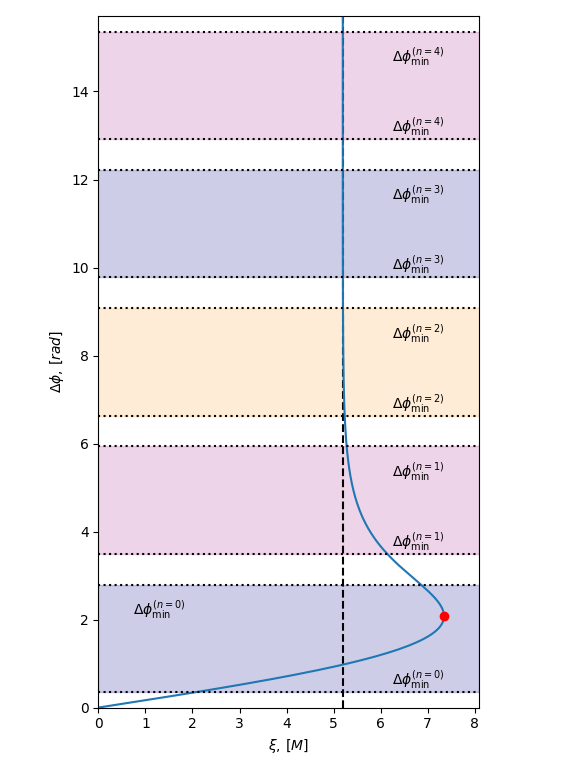
\includegraphics[scale = 0.5]{Schw_70_deg_ISCO_impact.png}
\captionof{figure}[$\Delta\phi(\xi)$ за ISCO орбитата на Шварцшилд при $i = 70^\circ$]{\small $\Delta\phi(\xi)$ за ISCO орбитата на Шварцшилд при $i = 70^\circ$. Всеки оцветен регион съответства на отделен образ на цялата орбита - т.е на решение на системата (6.6)}
\label{Scw_orbits_ISCO_impact_diagram}
\end{minipage}\,\,\,
\begin{minipage}{20em}
	Виждаме, че функцията $\Delta\phi(\xi)$ е съставена от два клона, разделени от точката P. Долният клон съответства на част от директният образ и представлява съвкупността от геодезични, свързващи наблюдателя и орбитата, които не достигат радиална точка на обръщане. Вертикалната асимптота съответства на критичния прицелен параметър $\xi_\text{crit} = -\sqrt{\frac{g_{\phi\phi}}{g_{tt}}}\big\vert_{r = r_\text{ph}}$, при който налитащите фотони попадат върху фотонната сфера. Тук можем да видим и известния факт, че с повишаване на $n$, образите на даден източник се "сплескват"$\,$ все повече към ръба на сянката. Имайки предвид израз (6.6б) виждаме, че ефективният размер на образа се определя от стойностите на $\xi_n$, който клони много бързо с $n$ към константната стойност $\xi_\text{crit}$. Това означава, че практически всички образи на даден източник са концентирани в много малък радиален диапазон отвъд сянката.
\end{minipage}\\

\begin{minipage}{20em}
На фигура \ref{Scw_orbits_ISCO_images} са начертани (с помощта на (6.6)) образи, съответстващи на фигура (6.1). Черната пунктирана линия съответства на ръба на сянката. Виждаме, че образите за които $n>1$ са на практика неразделими, ако наблюдаваме с характерна резолюция, съизмерима с радиуса на сянката.\\

\emph{Това е изключително важно за нашите изследвания, понеже показва, че за да наблюдаваме морфологични отклонения от стандартните черни дупки на Кер, те трябва да се проявят в образи от порядък по-нисък от $n = 2$.}
\end{minipage}\,\,\,
\begin{minipage}{16em}
	%\hspace{-0.5cm}
	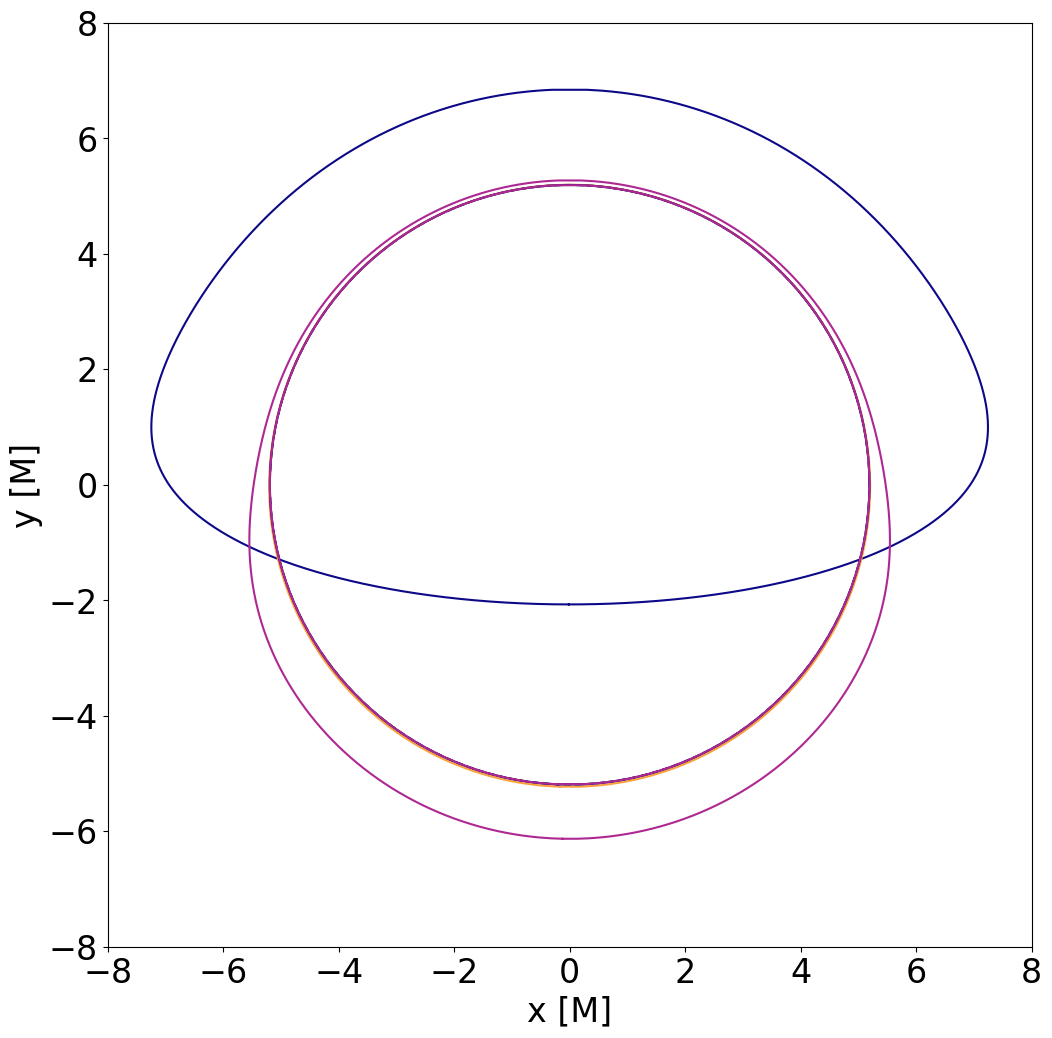
\includegraphics[scale = 0.3]{Schw_70_deg_ISCO.png}
	\captionof{figure}[Построени образи на ISCO орбитата на Шварцшилд при $i = 70^\circ$]{\small Образите на ISCO орбитата, съответстващи на решенията на системата (6.6) и на диаграмата $\Delta\phi(\xi)$ от фигура \ref{Scw_orbits_ISCO_impact_diagram}.}
	\label{Scw_orbits_ISCO_images}
\end{minipage}\\

На фигура \ref{Scw_r25_orbit} виждаме същото поведение на образите с увеличението на $n$, но за орбита с по-голям радиус $r_s = 25M$.

\begin{figure}[h]
	\centering
	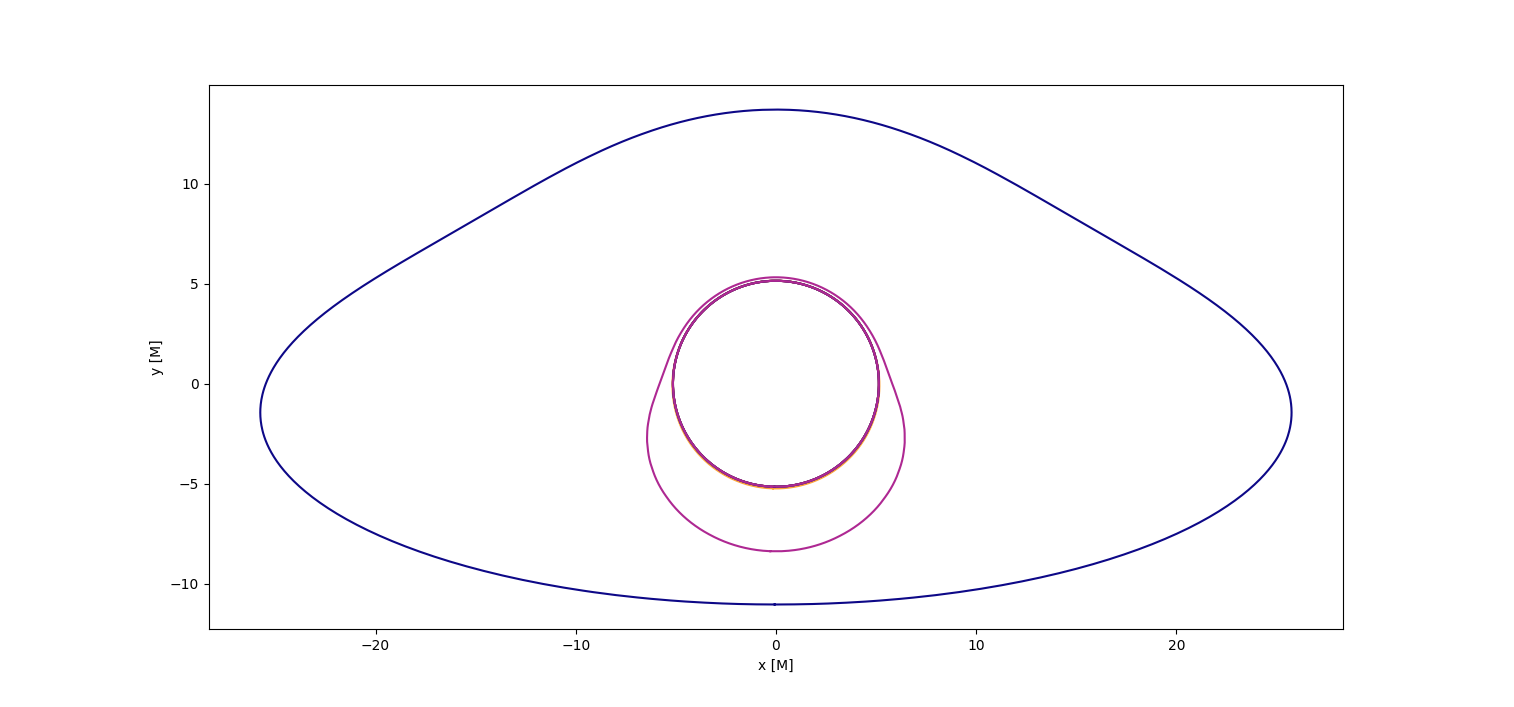
\includegraphics[scale = 0.3]{Schw_70_deg_r25.png}
	\caption[Конструиран образ на орбита с $r_s = 25M$ около черна дупка на Шварцшилд.]{\small Конструиран образ на орбита с $r_s = 25M$ около черна дупка на Шварцшилд $r_\text{obs} = 10^3M,\,\,i = 70^\circ$.} 
	\label{Scw_r25_orbit}
\end{figure}

В допълнение ДОПЪЛНЕНИЕ СРАВНЕИНЕ КОНТУРИ може да видим по-обстойно сравнение на образите на различни орбити при различни инклинации и метрични параметри.
\newpage

\subsubsection{Пространствено-времеви тунели}
Нека сега разгледаме същата орбита $r_s = 6M$, обаче наблюдавана около пространствено-времевия тунел от глава 5, при параметри $\gamma = 2,\,\, a = 0$ и същата инклинация на наблюдателя.
\begin{figure}[h]
	\centering
	\begin{subfigure}{6cm}
		\centering
		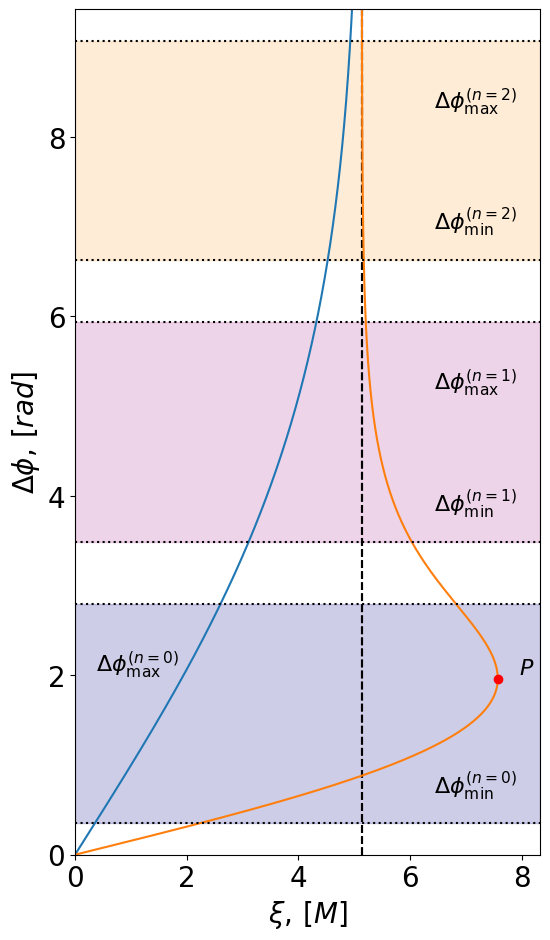
\includegraphics[scale = 0.3]{WH_70_deg_r6_impact_gamma_2.png}
		\caption{Решението на уравнение (6.5) $\Delta\phi(\xi)$ за двата типа траектории.} \label{fig:1a}
	\end{subfigure}\,\,\,
	\begin{subfigure}{6cm}
		\centering
		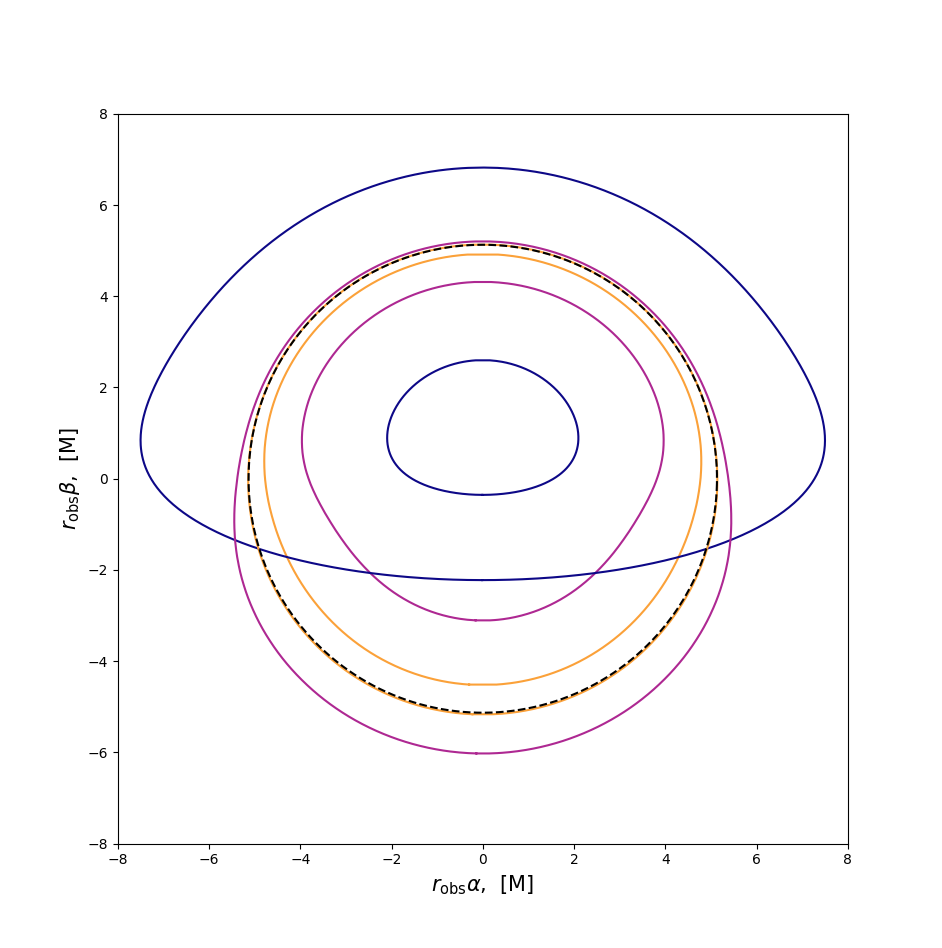
\includegraphics[scale = 0.3]{WH_70_deg_r6_gamma_2.png}
		\caption{Построени образи на база $\Delta\phi(\xi)$.\newline} \label{fig:1b}
	\end{subfigure}
	\caption[$\Delta\phi(\xi)$ и образите за $r_s=6M$ орбита около пространствено-времеви тунел до $n = 2$.]{\small $\Delta\phi(\xi)$ (а) и построените образите до $n = 2$ (б) за $r_s=6M$ орбита около пространствено-времеви тунел с параметри $\gamma = 2,\,\, a = 0$, и наблюдател с $r_\text{obs} = 10^3M,\,\,i = 70^\circ$. Черният контур съответства на границата на сянката.} 
	\label{WH_r6_orbit}
\end{figure}

\lfoot{}
Веднага можем да забележим значителна морфологична разлика спрямо черната дупка на Шварцшилд (фигура 6.2). Тук съществуват клас от фотони с прицелни параметри $\xi \le \xi_\text{crit}$ (синята крива от фигура 6.3а), които формират допълнителни образи, разположени \emph{вътре} в сянката. Те съответстват на орбитата $r_s = 6M$ от \emph{другата} страна на гърловината. Поради ниския си прицелен параметър, те минават под фотонната сфера и "попадат"$\,$ върху тунела, при което се разсейват от другата му страна, за да достигнат до наблюдателя. Наличието на симетрична фотонна сфера от двете страни на тунела генерира \emph{два} безкрайни набора от образи за всяка стойност на $n$. Можем да забележим също, че "новите"$\,$ образи клонят значително по-бавно към границата на сянката с увеличаването на $n$.\\

Тъй като от главен интерес за нас е възможността ни да наблюдаваме такива екзотични образи в бъдеще, нека изследваме очаквания размер на образа не на отделна орбита, ами на \emph{цялата} излъчваща среда. На фигура \ref{WH_img_size_deg} можем да видим контурите генерирани от екзотичните образи на орбити с радиус $r_s = \{6M, 500M\}$ за $n\in[0,2]$ и инклинации $i = \{20^\circ,70^\circ\}$.

\begin{figure}[!htb]
	\centering
	\begin{subfigure}{6cm}
		\hspace{-1.2cm}
		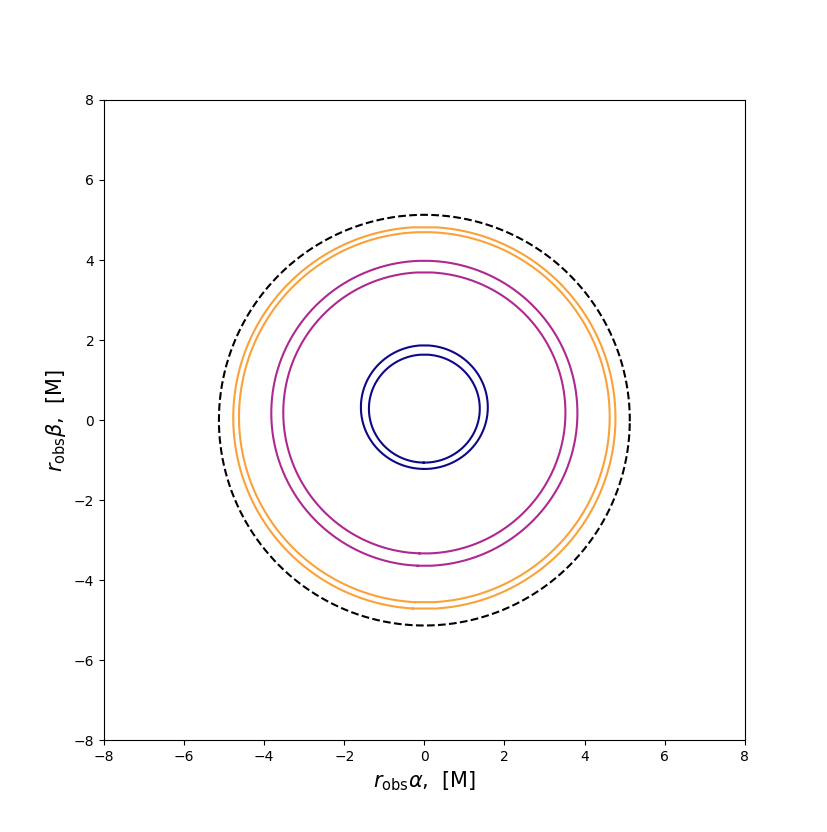
\includegraphics[scale = 0.35]{WH_20_deg_r6_r500.png}
		\caption{$r_s = \{6M, 500M\},\,\, i = 20^\circ$.}
	\end{subfigure}\,\,\,
	\begin{subfigure}{6cm}
		\hspace{-0.7cm}
		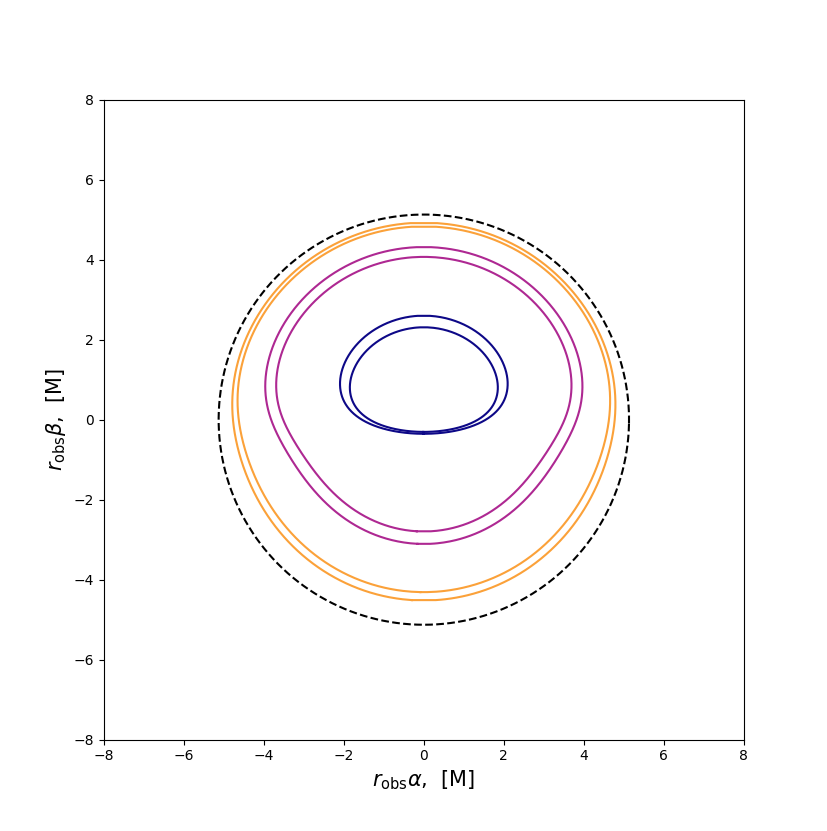
\includegraphics[scale = 0.35]{WH_70_deg_r6_r500.png}
		\caption{$r_s = \{6M, 500M\},\,\, i = 70^\circ$.}
	\end{subfigure}
	\caption[Характерните размери на екзотичните образите на цялата излъчваща среда, генерирани от пространствено-времеви тунел.]{\small Характерните размери на екзотичните образите на цялата излъчваща среда, генерирани от пространствено-времеви тунел. Черният контур съответства на сянката.} 
	\label{WH_img_size_deg}
\end{figure}
Виждаме, че директният образ, който за образи от "нашата"$\,$ страна на гърловината е отговорен за най-голямата част от наблюдаваният поток, е концентиран в много малък регион, вътре в сянката. Това подсказва, че тези екзотични образи имат потенциала да бъдат \emph{много интензивни}. В такъв случай те биха имали огромна наблюдателна релевантност. Ще изследваме това, използвайки модела на Новиков-Торн към края на тази глава.\\ 

Друг важен въпрос на който трябва да отговорим е дали тази пръстеновидна структура във вътрешността на сянката се запазва при различни стойности на параметъра $\gamma$. На фигура \ref{WH_gamma_70_deg} са показани същите $r_s = 6M$ орбити като на фигура \ref{WH_r6_orbit}, но за стойности на $\gamma =\{0, 3\}$. Докато на фигура \ref{WH_gamma_20_deg} са показани тези орбити от инклинация $i = 20^\circ$.
\newpage
\begin{figure}[!htb]
	\centering
	\begin{subfigure}{6cm}
		\hspace{-1.2cm}
		\includegraphics[scale = 0.35]{Wh_70_deg_r6_gamma_0.png}
		\caption{$r_s = 25M,\,\, i = 70^\circ,\,\,\gamma = 0$.} 
	\end{subfigure}\,\,\,
	\begin{subfigure}{6cm}
		\hspace{-0.7cm}
		\includegraphics[scale = 0.32]{Wh_70_deg_r6_gamma_3.png}
		\caption{$r_s = 6M,\,\, i = 70^\circ,\,\,\gamma = 3$.}
	\end{subfigure}
	\caption[Построени образи на $r_s = 6M$ орбита около пространствено-времеви тунел за различни стойности на $\gamma$ при $i \ 70^\circ$.]{\small Построени образи на $r_s = 6M$ орбита около пространствено-времеви тунел за стойности на $\gamma = \{0, 3\}$ при $i = 70^\circ$ и $n\in[0,10]$.} 
\label{WH_gamma_70_deg}
\end{figure}
\begin{figure}[!htb]
	\centering
	\begin{subfigure}{6cm}
		\hspace{-1.2cm}
		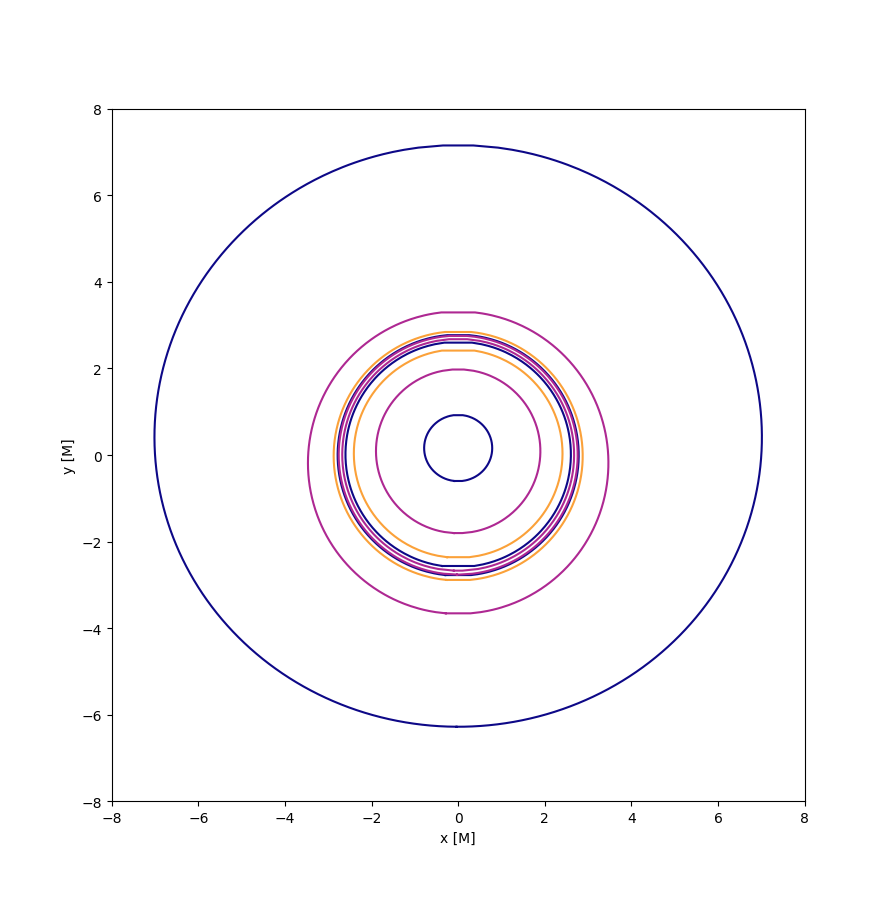
\includegraphics[scale = 0.32]{WH_20_deg_r6_gamma_0.png}
		\caption{$r_s = 6М,\,\, i = 20^\circ,\,\,\gamma = 0$.}
	\end{subfigure}\,\,\,
	\begin{subfigure}{6cm}
		\hspace{-0.7cm}
		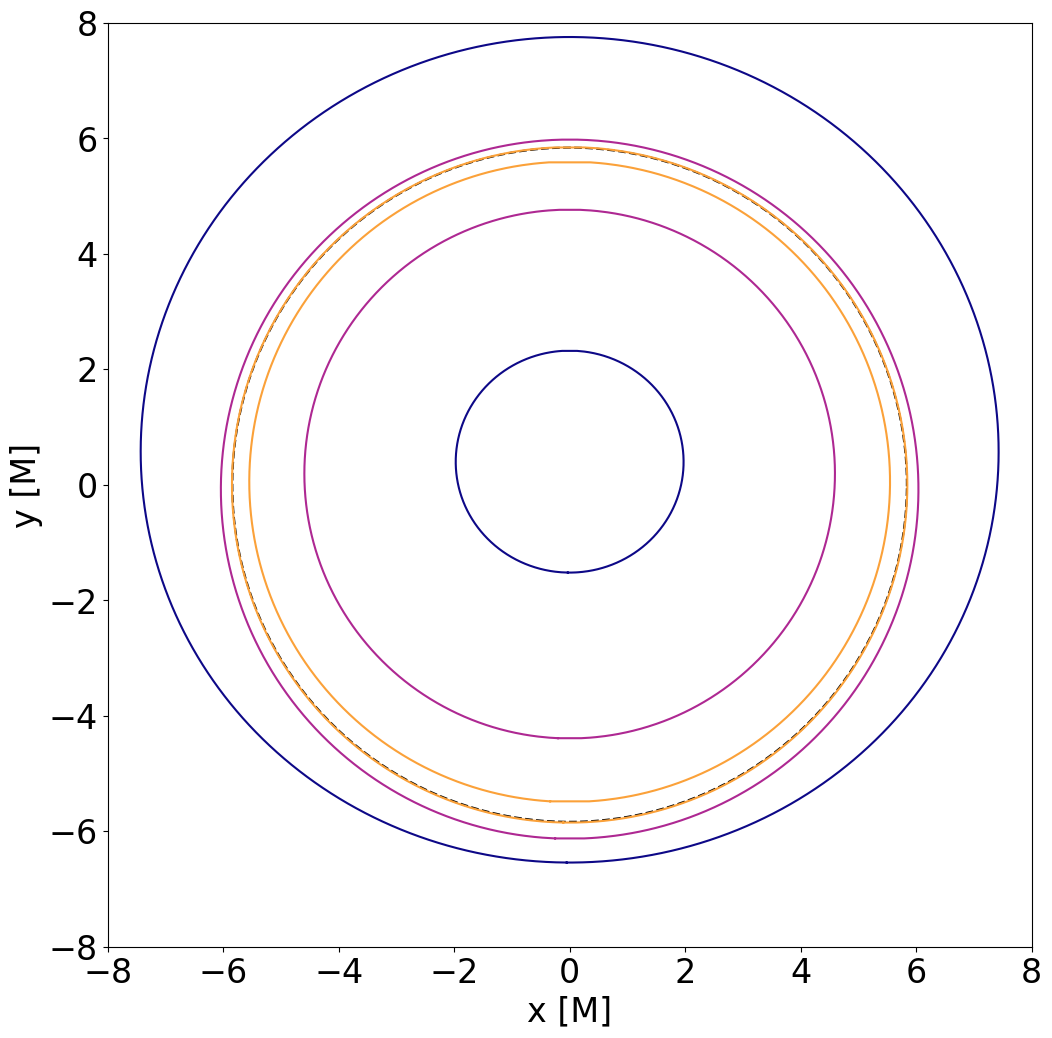
\includegraphics[scale = 0.32]{WH_20_deg_r6_gamma_3.png}
		\caption{$r_s = 6M,\,\, i = 20^\circ,\,\,\gamma = 3$.}
	\end{subfigure}
	\caption[Построени образи на $r_s = 6M$ орбита около пространствено-времеви тунел за различни стойности на $\gamma$ при $i \ 20^\circ$.]{\small Построени образи на $r_s = 6M$ орбита около пространствено-времеви тунел за стойности на $\gamma = \{0, 3\}$ при $i = 40^\circ$ и $n\in[0,4]$.} 
	\label{WH_gamma_20_deg}
\end{figure}
На база на това можем да смятаме пръстеновидната структура като общ характерен белег за този тип компактен обект (виж също допълнение ДОПЪЛНЕНИЕ СРАВНЕНИЕ), чието евентуално наблюдателно засичане би дало ясна индикация, че пространство-времето около този обект е силно различно от това на Кер.
\newpage
\subsubsection{Голи сингулярности на Джанис-Нюман-Уиникър}

Нека сега разгледаме образите генерирани от тази гола сингулярност в слабия режим $\gamma\in\left[\frac{1}{2},1\right]$, където тя притежава фотонна сфера. За разлика от пространствено времевите тунели, при тази сингулярност, в присъствието на фотонна сфера, всички фотони с прицелни параметри $\xi <\xi_\text{crit} = \sqrt{-\frac{g_{\phi\phi}}{g_{tt}}}\big\vert_{r = r_\text{ph}}$ завършват върху сингулярността. Това можем да видим от графиката на ефективния потенциал $V_\text{eff}$, участваш в уравнение (6.4а):

\begin{minipage}{18em}
	\hspace{-0.5cm}
	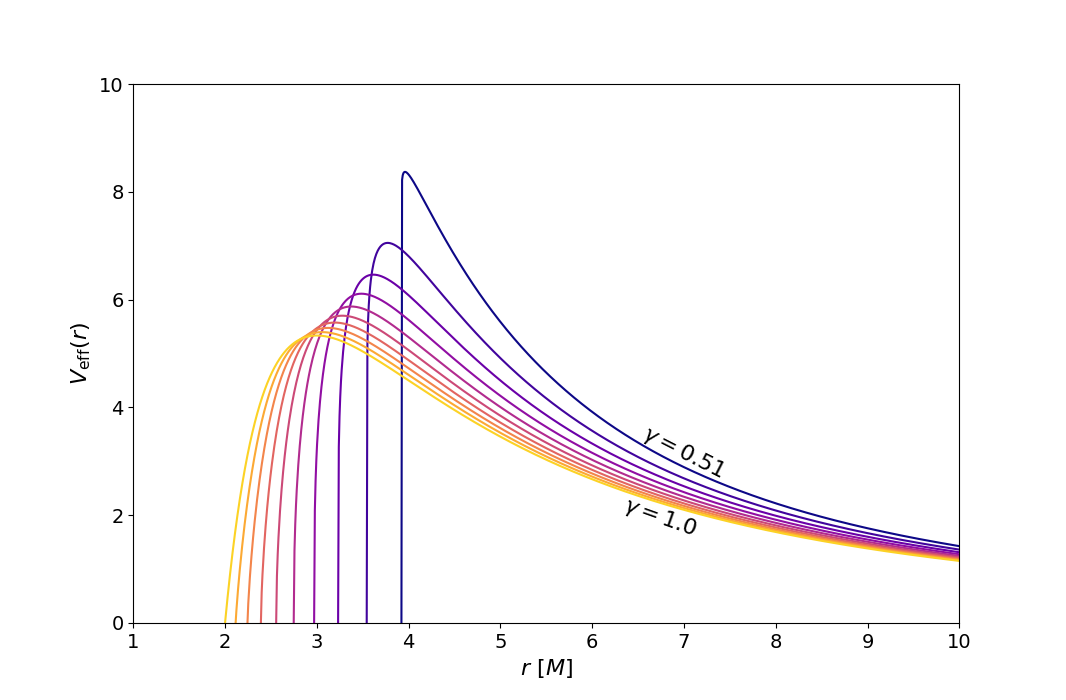
\includegraphics[scale = 0.3]{JNW_eff_potential_photon_sphere.png}
	\caption[Ефективният потенциал за слаби сингуларности на Джанис-Нюман-Уиникър]{Ефективният потенциал $V_\text{eff}$ за слаби сингуларности на Джанис-Нюман-Уиникър при избрани стойности на $\gamma > \frac{1}{2}$ и $\xi = 12M$.}
\end{minipage}\,\,
\begin{minipage}{18em}
	Виждаме, че качественото поведение на потенциала е същото като при черни дупки на Шварцшилд $\gamma = 1$. Следователно не очакваме в този режим да има "отразени"$\,$ фотони, които да достигнат обратно до наблюдателя и да генерират допълнителни образи. На фигура \ref{JNW_r6_70_deg} можем да видим построените образи на орбитата $r_s = 6M$ за стойности на $\gamma = \{0.52, 0.8\}$. Сравнявайки с фигура 6.2 виждаме качествено същата картинка.
\end{minipage}
\begin{figure}[!htb]
	\centering
	\begin{subfigure}{6cm}
		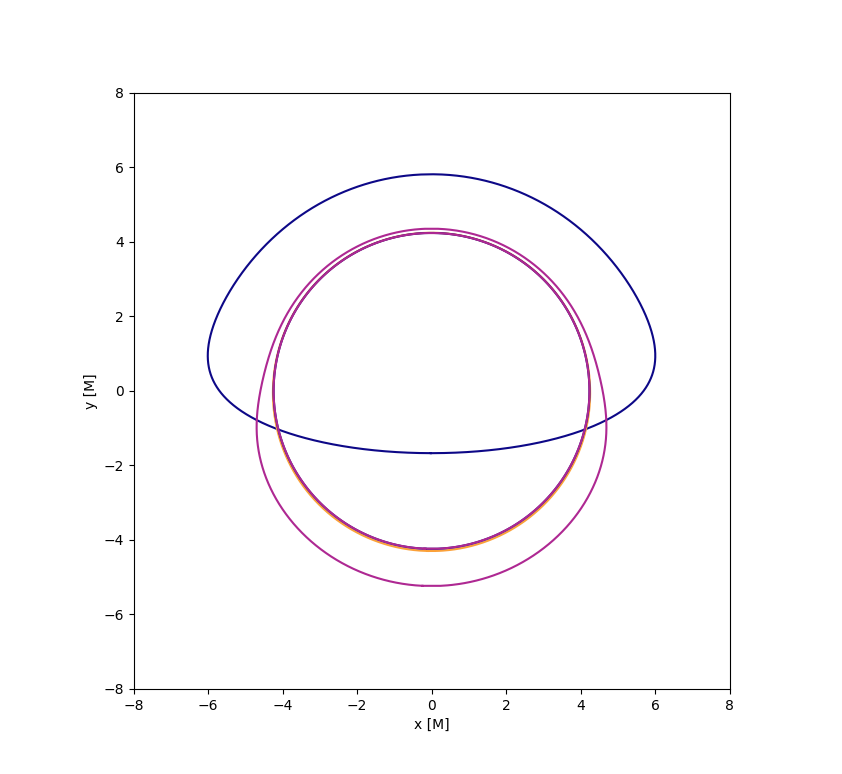
\includegraphics[scale = 0.3]{JNW_70_deg_r6_gamma_0.52.png}
		\caption{$r_s = 6M,\,\, i = 70^\circ,\,\,\gamma = 0.52$.} 
	\end{subfigure}\,\,\,
	\begin{subfigure}{6cm}
		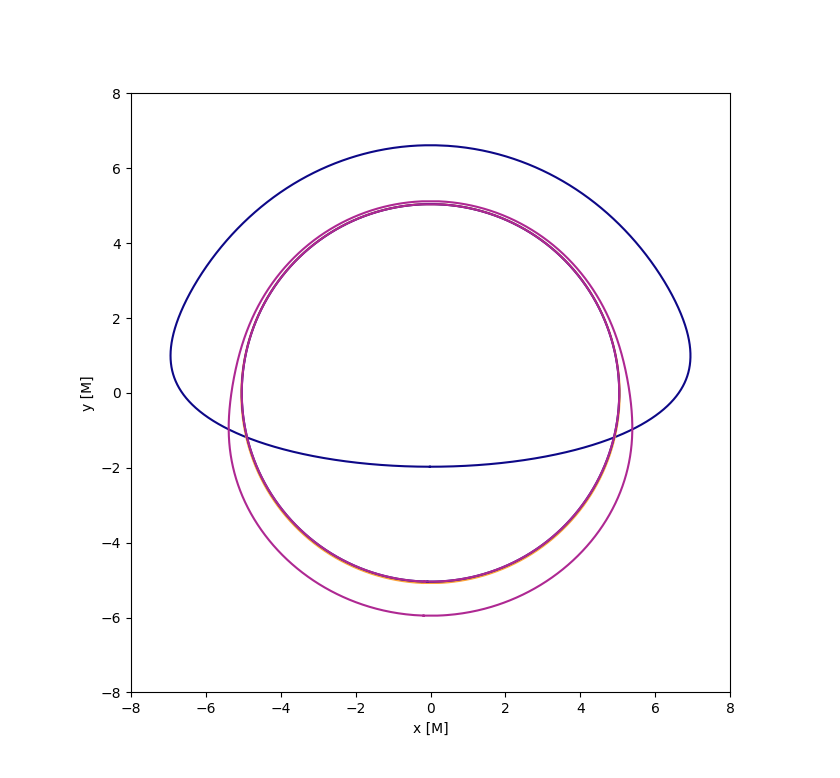
\includegraphics[scale = 0.3]{JNW_70_deg_r6_gamma_0.8.png}
		\caption{$r_s = 6M,\,\, i = 70^\circ,\,\,\gamma = 0.8$.}
	\end{subfigure}
	\caption[Построени образи на $r_s = 6M$ орбита около слаба гола сингулярност на Джанис-Нюман-Уиникър за различни стойности на $\gamma$ при $i = 70^\circ$.]{\small Построени образи на $r_s = 6M$ орбита около слаба гола сингулярност на Джанис-Нюман-Уиникър за стойности на $\gamma = \{0.52, 0.80\}$ при $i = 70^\circ$ и $n\in[0,4]$.} 
	\label{JNW_r6_70_deg}
\end{figure}

Виждаме, че единствената морфологична разлика е характерният размер на образите - за намаляващи $\gamma$, той също намалява. Също така виждаме липса на екзотични образи, които нямат еквивалент за черни дупки на Шварцшилд. Това не се променя и при ниски инклинации (фигура \ref{JNW_r6_20_deg}).

\begin{figure}[!htb]
	\centering
	\begin{subfigure}{6cm}
		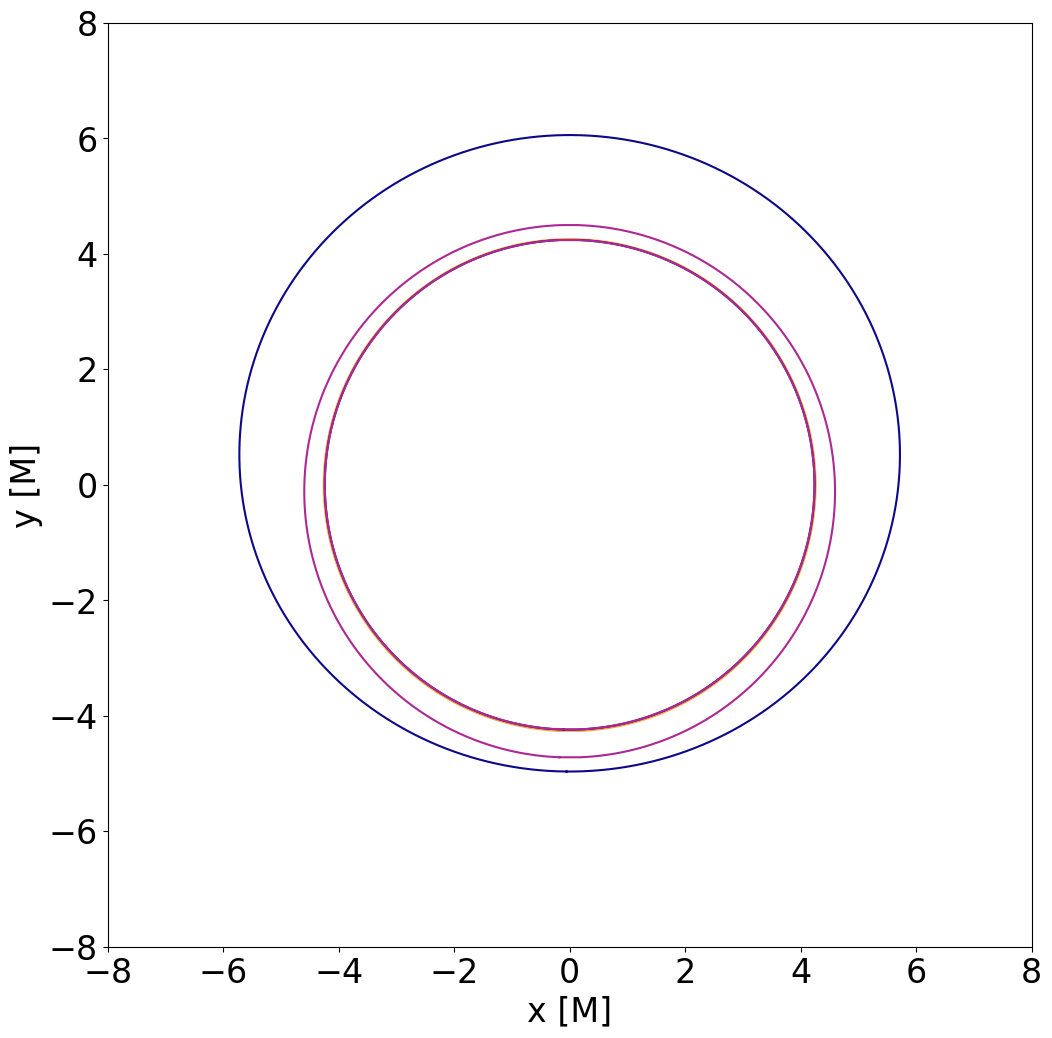
\includegraphics[scale = 0.3]{JNW_20_deg_r6_gamma_0.52.png}
		\caption{$r_s = 6M,\,\, i = 20^\circ,\,\,\gamma = 0.52$.} 
	\end{subfigure}\,\,\,
	\begin{subfigure}{6cm}
		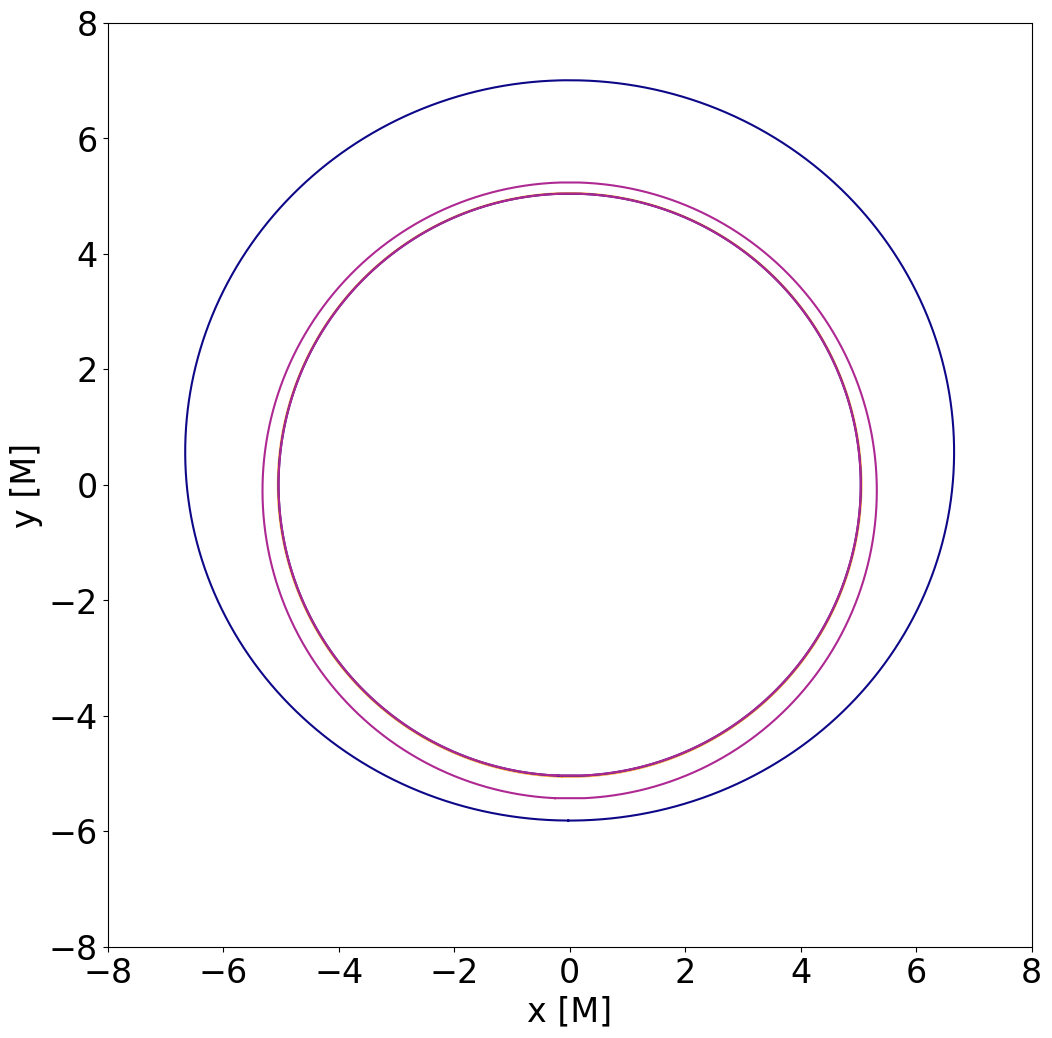
\includegraphics[scale = 0.3]{JNW_20_deg_r6_gamma_0.8.png}
		\caption{$r_s = 6M,\,\, i = 20^\circ,\,\,\gamma = 0.8$.}
	\end{subfigure}
	\caption[Построени образи на $r_s = 6M$ орбита около слаба гола сингулярност на Джанис-Нюман-Уиникър за различни стойности на $\gamma$ при $i = 20^\circ$.]{\small Построени образи на $r_s = 6M$ орбита около слаба гола сингулярност на Джанис-Нюман-Уиникър за стойности на $\gamma = \{0.52, 0.80\}$ при $i = 20^\circ$ и $n\in[0,4]$.} 
	\label{JNW_r6_20_deg}
\end{figure}

Следователно определяме слабата гола сингулярност на Джанис-Нюман-Уиникър като \emph{имитатор} на черна дупка на Шварцшилд от гледна точка на морфологията на образите ѝ. Това е в контраст на \emph{силният} режим на този обект, който ще обсъдим в подточка 6.3.

\subsubsection{Решение на Гаус-Боне} 
Както видяхме в подточка 3 на глава 5, този обект притежава фотонна сфера за стойности на параметъра $\gamma\in\left(1,\frac{3\sqrt{3}}{4}\right)$. За разлика от голите сингулярности на Джанис-Нюман-Уиникър, тук ефективният потенциал $V_\text{eff}$ е положително разходящ в околност на сингулярността $r = 0$ (фигура \ref{GB_eff_pot}).

\begin{minipage}{18em}
	\centering
	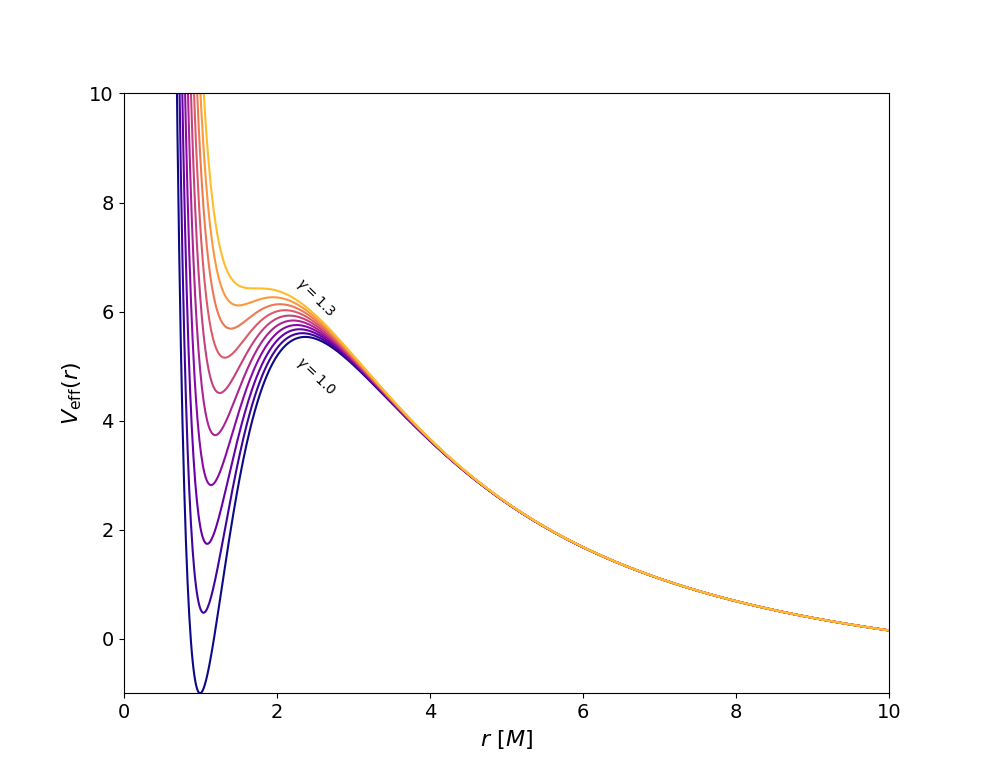
\includegraphics[scale = 0.3]{GB_eff_potential.png}
	\caption[Ефективният потенциал за слаби сингуларности на Гаус-Боне]{Ефективният потенциал $V_\text{eff}$ за слаби сингуларности на Гаус-Боне при избрани стойности на $\gamma\in\left[1, \frac{3\sqrt{3}}{4}\right]$ и $\xi = 12M$.}
	\label{GB_eff_pot}
\end{minipage}\,\,
\begin{minipage}{18em}
	Виждаме, че качественото потенциалът е разходящ в околност на $r = 0$ и следователно можем да очакваме фотони да бъдат отразени от този регион и да достигнат наблюдателя. Ще се ограничим до стойности на $\gamma > 1$ понеже в интервала $\gamma \in \left[0,1\right]$ разходящият регион на потенциала се намира \emph{под} хоризонта на събитията $r_h = 1 +\sqrt{M^2 - \gamma}$. На фигура \ref{GB_r6_20_deg_gamma_1} можем да видим, че в този интервал на $\gamma$ решението на Гаус-Боне също "имитира"$\,$ черна дупка на Шварцшилд.
\end{minipage}
\newpage

\begin{figure}[!htb]
	\centering
	\begin{subfigure}{6cm}
		\centering
		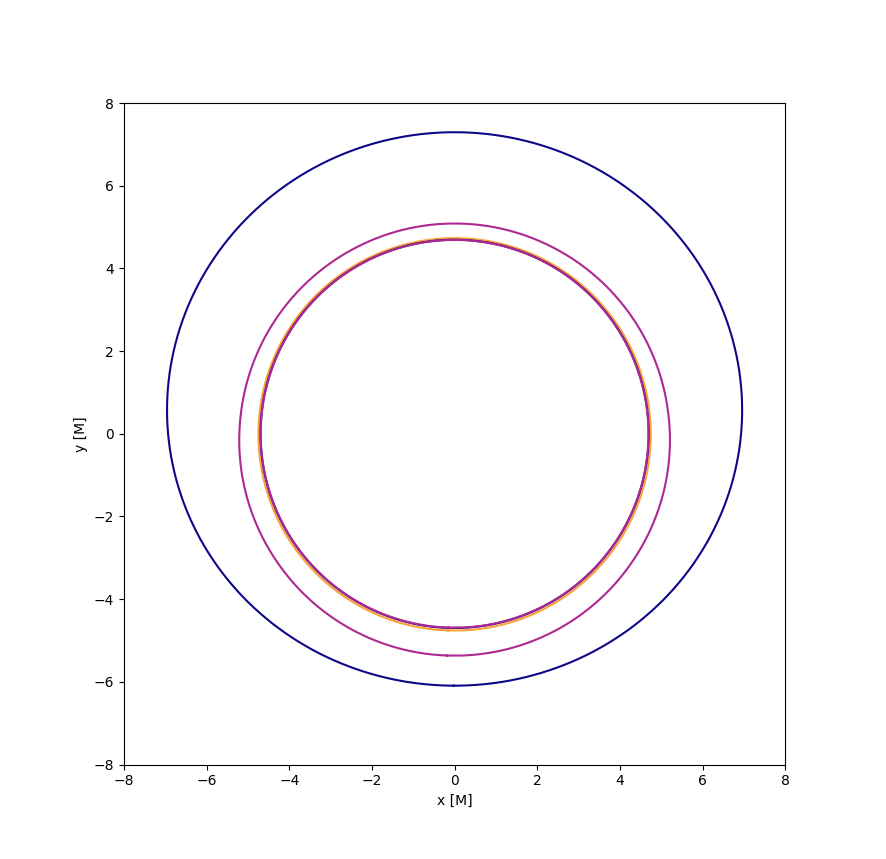
\includegraphics[scale = 0.3]{GB_20_deg_r6_gamma_1.png}
		\caption{$r_s = 6M,\,\, i = 20^\circ,\,\,\gamma = 1.0$.} 
	\end{subfigure}\,\,\,
	\begin{subfigure}{6cm}
		\centering
		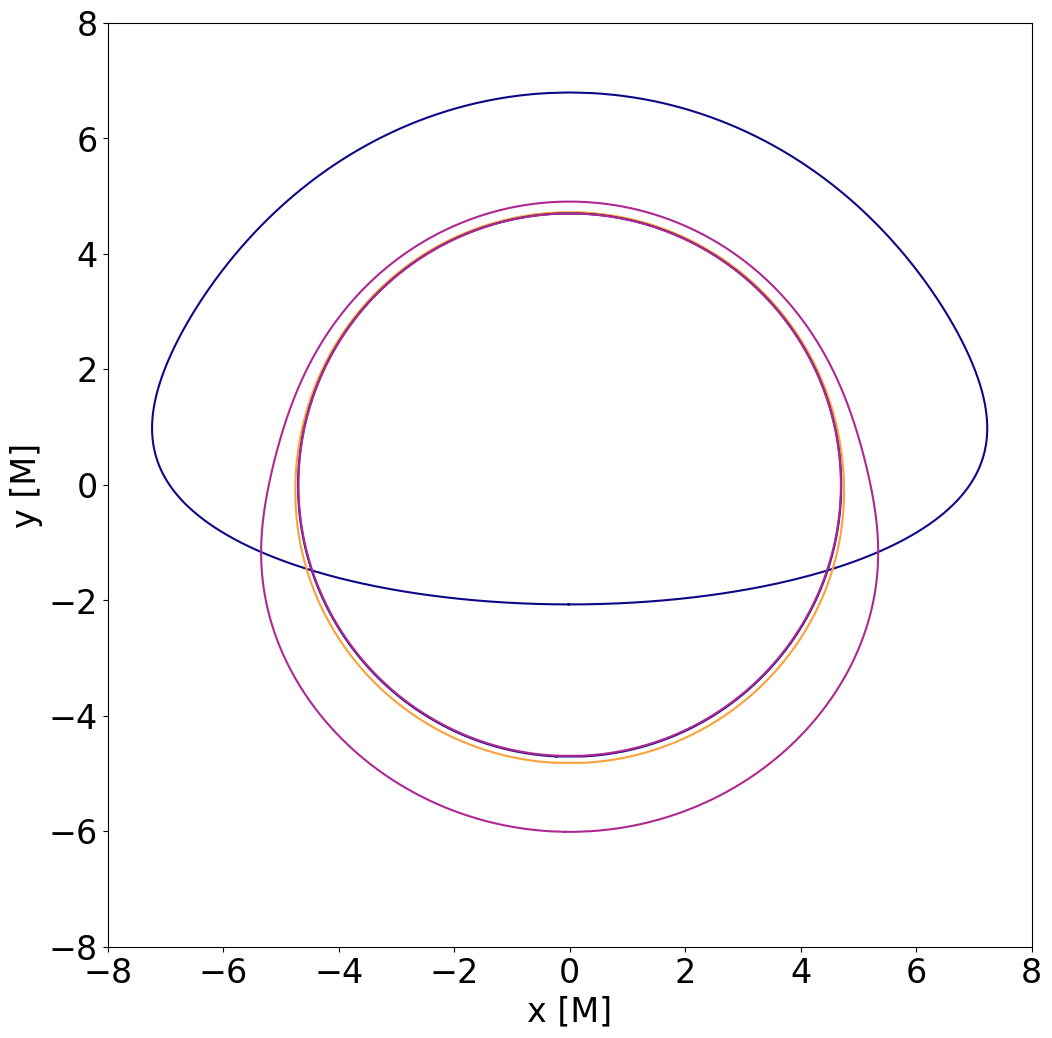
\includegraphics[scale = 0.3]{GB_70_deg_r6_gamma_1.png}
		\caption{$r_s = 6M,\,\, i = 70^\circ,\,\,\gamma = 1.0$.} 
	\end{subfigure}
	\caption[Построени образи на $r_s = 6M$ орбита около черна дупка на Гаус-Боне за различни инклинации.]{\small Построени образи на $r_s = 6M$ орбита около черна дупка на Гаус-Боне за $\gamma = 1.0$ при $i = \{20^\circ, 70^\circ\}$ и $n\in[0,4]$.} 
	\label{GB_r6_20_deg_gamma_1}
\end{figure}

Поведението на образите се променя драстично обаче, за стойности на $\gamma > 1$, когато решението описва гола сингулярност. Тогава разходящите региони на потенциала не са "скрити"$,$ зад хоризонт и фотони могат да се разсеят от тях и да достигнат наблюдател на безкрайност. Това е показано на фигура \ref{GB_r6_70_deg_gamma_1.15} за $\gamma = 1.15$.

\begin{figure}[!htb]
	\centering
	\begin{subfigure}{6cm}
		\hspace{0.8cm}
		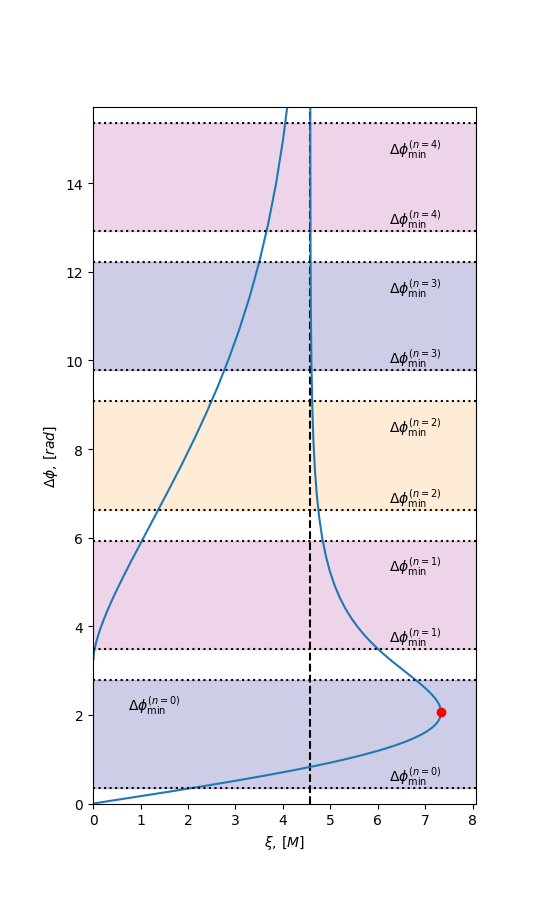
\includegraphics[scale = 0.32]{GB_70_deg_r6_gamma_1.15_impact.png}
		\caption{Решението $\Delta\phi(\xi)$ за $r_s = 6M,\,\, i = 70^\circ,\,\,\gamma = 1.15$.} 
	\end{subfigure}\,\,\,
	\begin{subfigure}{6cm}
		\hspace{-0.5cm}
		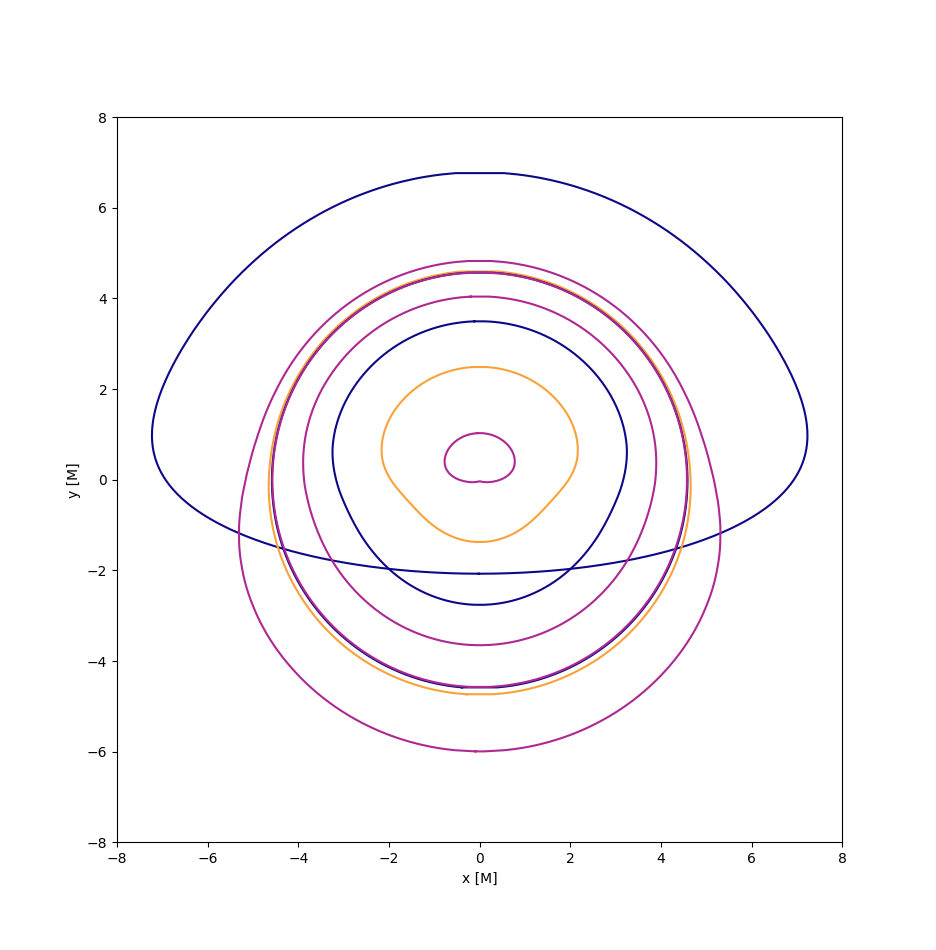
\includegraphics[scale = 0.3]{GB_70_deg_r6_gamma_1.15.png}
		\caption{Построени образи на база на  $\Delta\phi(\xi)$.} 
	\end{subfigure}
	\caption[Построени образи на $r_s = 6M$ орбита около гола сингулярност на Гаус-Боне за $i = 70^\circ$.]{\small Построени образи на $r_s = 6M$ орбита около гола сингуларност на Гаус-Боне за $\gamma = 1.15$ при $i = 70^\circ$ и $n\in[0,4]$.} 
	\label{GB_r6_70_deg_gamma_1.15}
\end{figure}

Виждаме, че диаграмата на $\Delta\phi(\xi)$ изглежда по качествено същият начин като фигура \ref{WH_r6_orbit}a. За разлика от там обаче, тука левият клон, съответстващ на прицелни параметри $\xi < \xi_\text{crit}$ не се дължи на фотони, преминаващи през регулярен тунел, а на такива които се разсейват от сингулярността. Въпреки, че природата на този клон от решението $\Delta\phi(\xi)$ е драстично различен, феноменологията на генерираните екзотични образи е сходна. На фигура \ref{GB_img_size_deg} можем да видим оценка на размера на тези екзотични образи. Също като фигура \ref{WH_img_size_deg}, и тук те са ограничени до много малък регион, вътре в сянката на сингулярността, което подсказва, че имат потенциалът да са силно интензивни и следователно наблюдателно релевантни.

\begin{figure}[!htb]
	\centering
	\begin{subfigure}{6cm}
		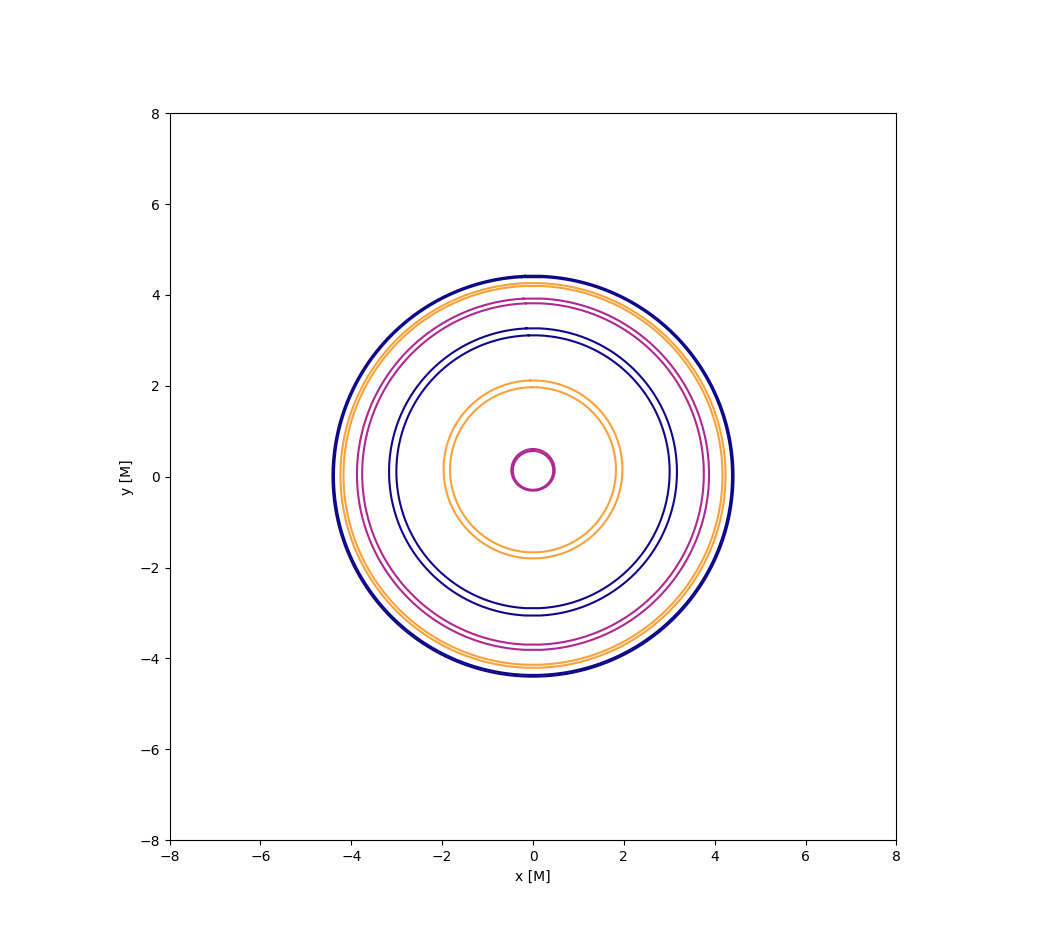
\includegraphics[scale = 0.25]{GB_20_deg_r6_500_gamma_1.15.png}
		\caption{$r_s = \{6M, 500M\},\,\, i = 20^\circ$.}
	\end{subfigure}\,\,\,
	\begin{subfigure}{6cm}
		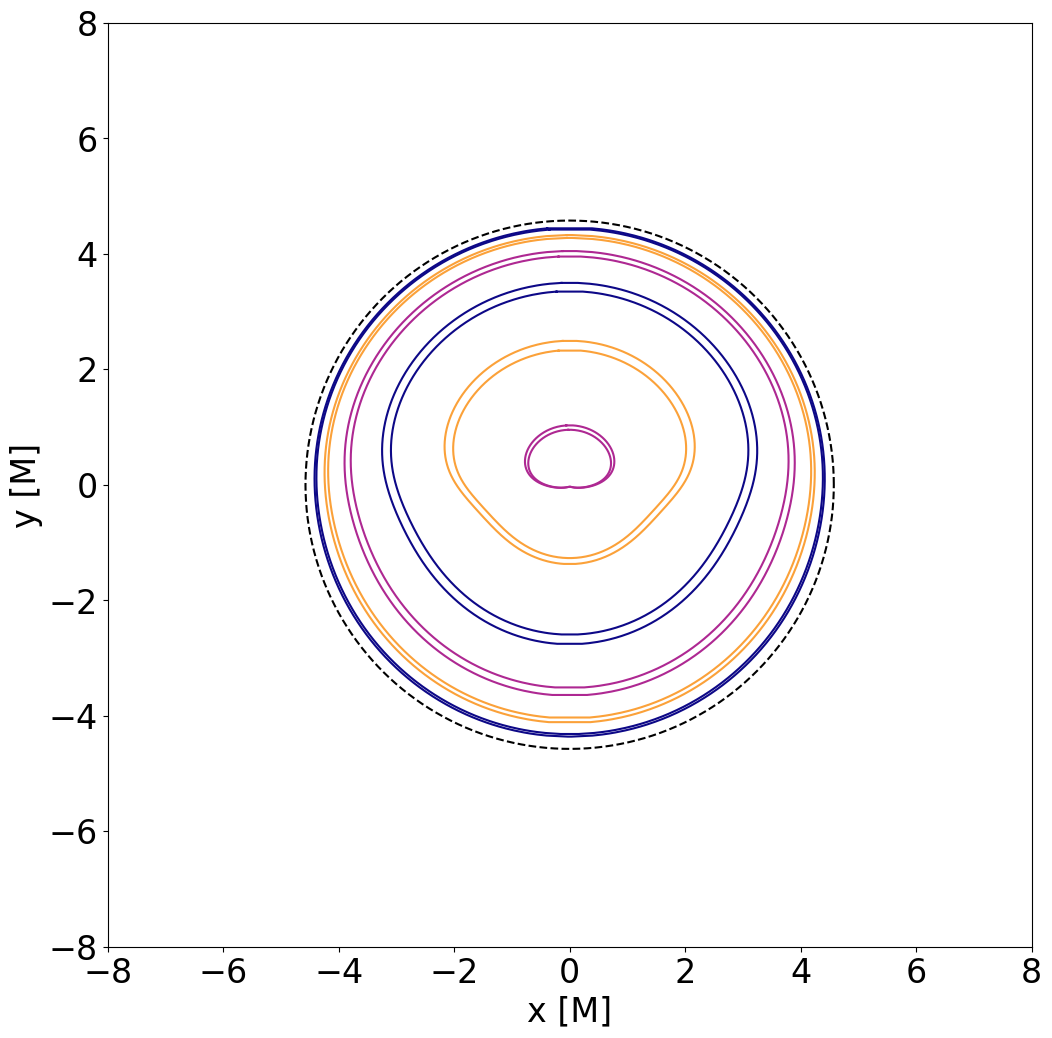
\includegraphics[scale = 0.25]{GB_70_deg_r6_500_gamma_1.15.png}
		\caption{$r_s = \{6M, 500M\},\,\, i = 70^\circ$.}
	\end{subfigure}
	\caption[Характерните размери на екзотичните образите на цялата излъчваща среда, генерирани от гола сингулярност на Гаус-Боне.]{\small Характерните размери на екзотичните образите на цялата излъчваща среда, генерирани от гола сингулярност на Гаус-Боне за $n\in[0, 4]$.} 
	\label{GB_img_size_deg}
\end{figure}

\subsection{Образи, генерирани при липса на фотонна сфера}

Двете обсъдени голи сингулярности могат да съществуват в режим, при който \emph{не} допускат съществуването на фотонна сфера. Това има драстичен ефект върху морфологията на генерираните от тях образи. От феноменологична гледна точка, многократното "навиване"$\,$ на фотоните около компактният обект, отговорно за генерирането на безкрайният набор от пръстени, видян в горните фигури, в този режим е невъзможно. Това подсказва, че броят генерирани образи в този режим е \emph{органичен отгоре}. Това можем да видим да фигура асфаса, където са представени образите на $r_s = 6M$ орбита около гола сингулярност на Джанис-Нюман-Уиникър (в, г) за $\gamma = 0.48$ и тази на Гаус-Боне (а, б) за $\gamma = 1.35$ при $i = 70^\circ$. Докато на фигура \ref{JNW_r25} е представена $r_s = 25M$ орбита при $i = 80^\circ$ около гола сингуларност на Джанис-Нюман-Уиникър, отново за $\gamma = 0.48$. \newpage

\begin{figure}[!htb]
	\centering
	\begin{subfigure}{6cm}
		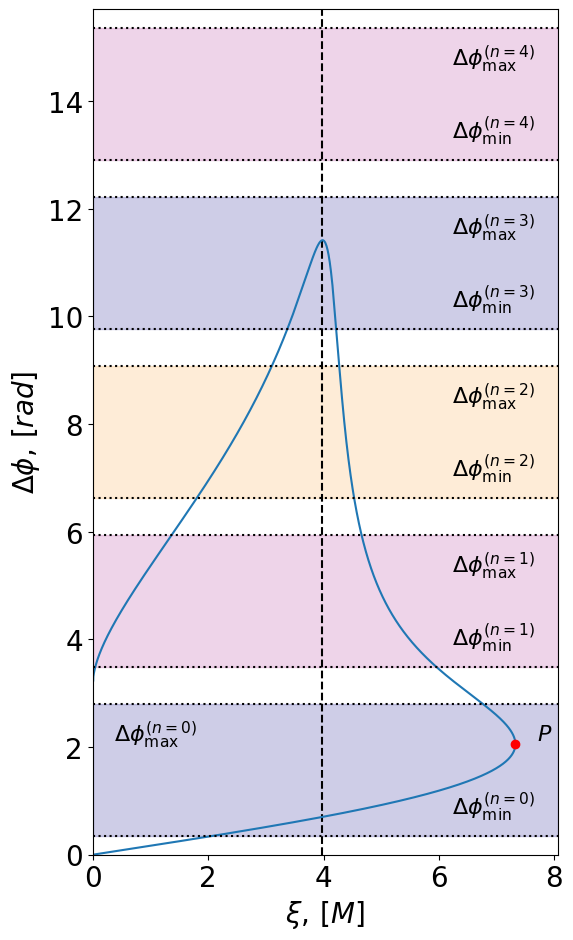
\includegraphics[scale = 0.32]{GB_70_deg_r6_gamma_1.5_impact.png}
		\caption{Решението $\Delta\phi(\xi)$ за $r_s = 6M,\,\, i = 20^\circ,\,\,\gamma = 1.5$.} 
	\end{subfigure}\,\,\,
	\begin{subfigure}{6cm}
		\hspace{-0.8cm}
		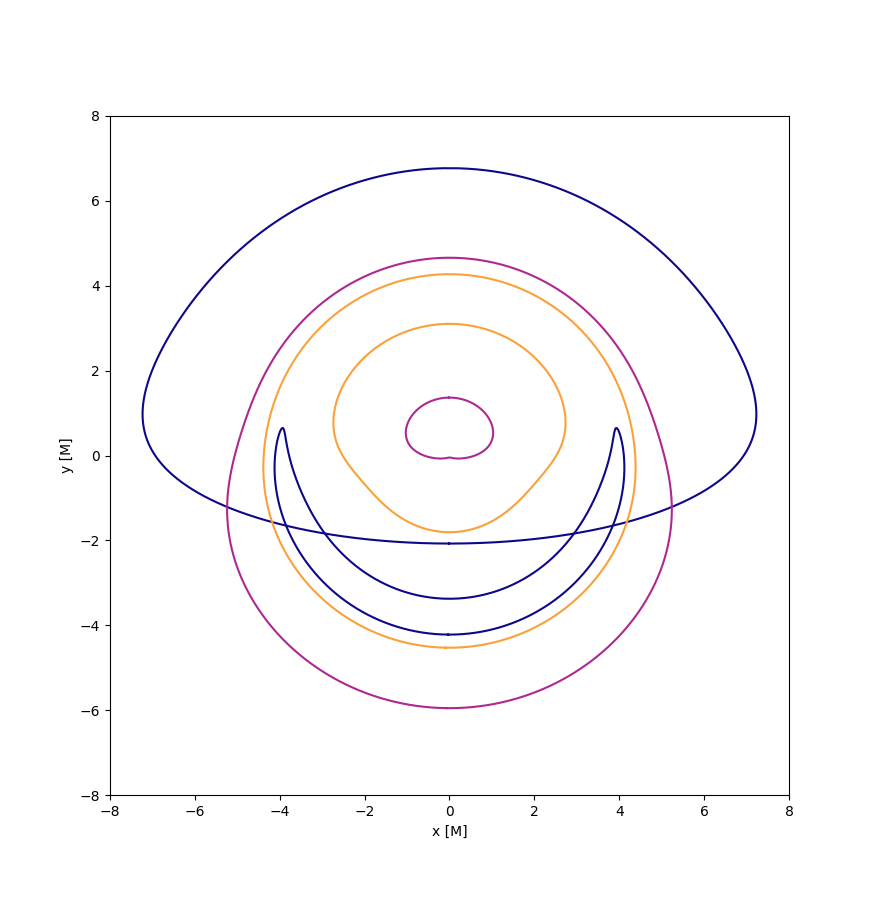
\includegraphics[scale = 0.3]{GB_70_deg_r6_gamma_1.5.png}
		\caption{Построени образи на база на  $\Delta\phi(\xi)$.} 
	\end{subfigure}
	\begin{subfigure}{6cm}
		\hspace{0.8cm}
		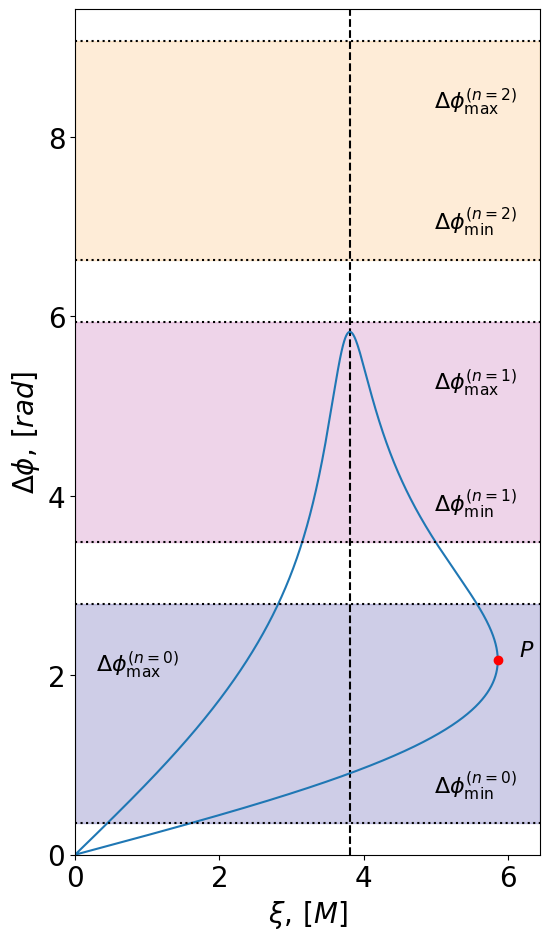
\includegraphics[scale = 0.32]{JNW_70_deg_r6_gamma_0.48_impact.png}
		\caption{Решението $\Delta\phi(\xi)$ за $r_s = 6M,\,\, i = 70^\circ,\,\,\gamma = 0.48$.} 
	\end{subfigure}\,\,\,
	\begin{subfigure}{6cm}
		\hspace{-0.5cm}
		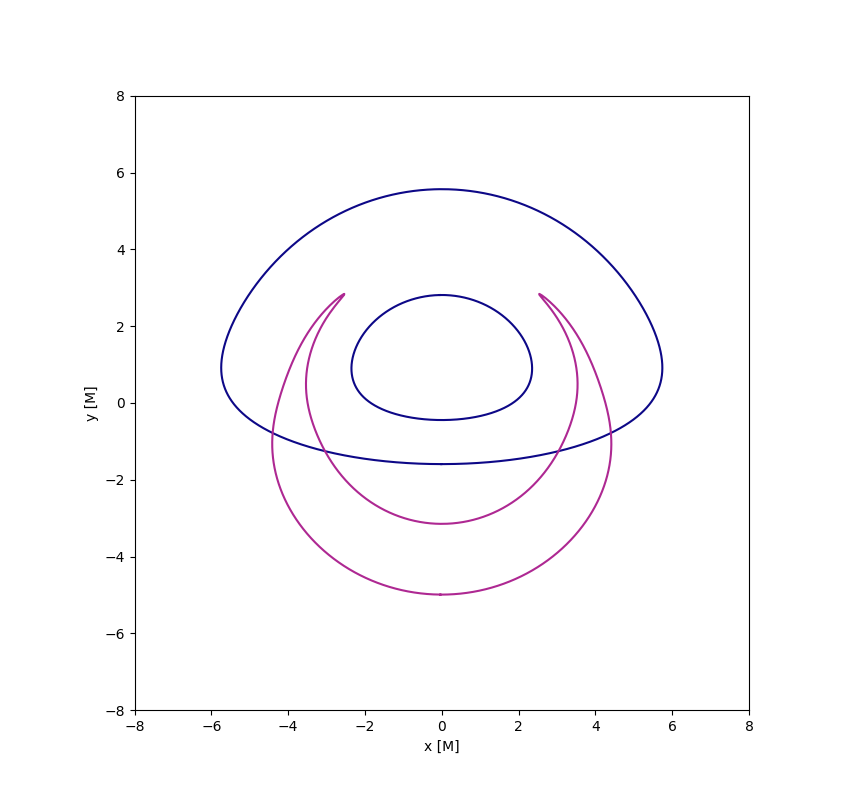
\includegraphics[scale = 0.3]{JNW_70_deg_r6_gamma_0.48.png}
		\caption{Построени образи на база на  $\Delta\phi(\xi)$.} 
	\end{subfigure}
	\caption[Построени образи на $r_s = 6M$ орбита около синлни голи сингулярности.]{\small Построени образи на $r_s = 6M$ орбита около синлни голи сингулярности на $r_s = 6M$ при $i = \{70^\circ, 70^\circ\}$.} 
	\label{GB_JNW_r6}
\end{figure}
\begin{figure}
	\centering
	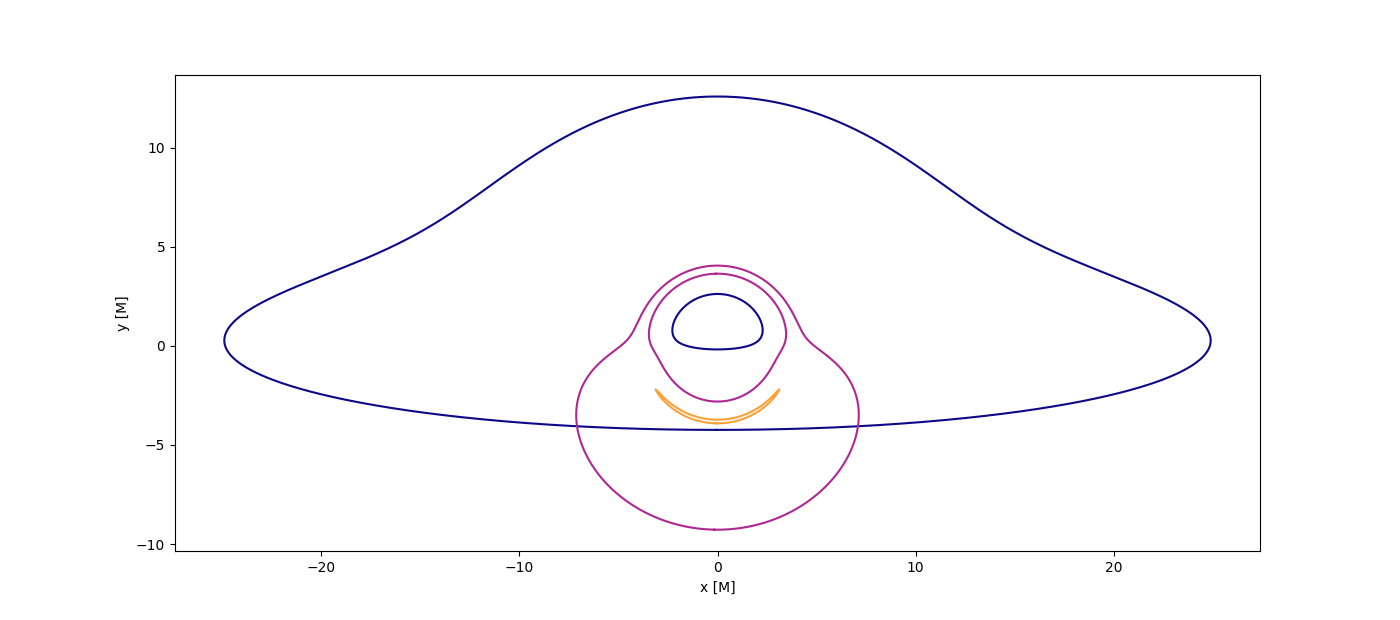
\includegraphics[scale = 0.35]{GB_70_deg_r25_gamma_0.48.png}
	\caption[Построени образи на $r_s = 25M$ орбита около синлни гола сингулярност на Джанис-Нюман-Уиникър.]{\small Построени образи на $r_s = 25M$ орбита около силна гола сингулярност на Джанис-Нюман-Уиникър при $i = 80^\circ$.} 
	\label{JNW_r25}
\end{figure}
Виждаме, че наистина липсата на фотонна сфера ограничава отгоре $\Delta\phi$, което води до краен максимум на графиките \ref{GB_JNW_r6}a и \ref{GB_JNW_r6}в. Ако той попадне вътре в някой от цветните региони, съответстващи на решение на системата (6.6), това съответства на образи, които не се "затварят"$\,$ около $x = y = 0$. Това поведение е силно характерно за пространства, които не притежават фотонна сфера и също може да служи като силен наблюдателен белег.
\newpage
\subsection{Наблюдателна релевантност на екзотичните образи}

Сега нека се фокусираме върху относителният поток, който можем да очакваме да наблюдаваме от тези образи. За тази цел ще използваме модела на безкрайно тънък, оптически плътен диск. Както коментирахме в увода, удобството на този модел е, че зависи единствено от метриката и два свободни параметъра - вътрешният $r_\text{in}$ (който ние ще фиксираме на $r_\text{ISCO}$) и външният $r_\text{out}$ радиус на диска. За подробна дискусия по самия модел насочваме читателя към CITE THORNE HERE. Накратко:\\

Моделът предполага аксиално (и в частност сферично) симетрично пространство-време и моделира диска като аксиално симетричен, чието усреденено по времето движение е чисто екваториално. Дискът се приема за \emph{тънък} - т.е. с характерна дебелина във всяка точка $2h \ll r$ и се приема, че единственият значим поток на енергия, напускащ диска е под формата на електромагнитно лъчение от повърхността му. Пренебрегват се ефекти на конвекция, или нагряване вследствие на поглъщане на лъчение от други части на диска.\\

Релевантното за нас предсказание на този модел е следното: Пълният поток $F$ в точката $\{t,r,\theta,\phi\}$ (енергия за единица време от единица площ, измерен от наблюдател, движещ се със средната скорост на излъчващата среда в тази точка) зависи само от радиалната координата се дава с изразът:
\begin{equation}
	F(r) = - \frac{\dot{M}}{4\pi\sqrt{-g^{(3)}}}\frac{\partial_r\Omega}{\left(E - \Omega L_z\right)^2}\int_{r_\text{ISCO}}^r \left(E - \Omega L_z\right)\partial_rL_zdr^\prime,
\end{equation}
където $E = E(r)$, $L_z = L_z(r)$ и $\Omega = \Omega(r)$ са усреднените по времето енергия, момент на импулса и ъгловат скорост на излъчващата среда в точката $\{t,r\theta,\phi\}$ (задавани от изрази ДОПЪЛНЕНИЕ), докато $g^{(3)}$ е детерминантата на индуцираната метрика в екваториалната равнина. Тъй като това е поток, измерен от наблюдател, движещ се заедно със средата, е нужно той да бъде пренесен до наблюдател на безкрайност. Това става посредством червеното отместване $(1 + z)^{-1}$. Тогава потокът $\mathcal{F}$, измерен от наблюдател в точката $\vec{r}_{\text{obs}}$ е:
\begin{equation}
	\mathcal{F}(r,\phi) = \left(\frac{1}{1+z} \right)^4 F(r),\quad \frac{1}{1 + z} = \frac{k_\mu v^\mu\vert_{\vec{r} = \vec{r}_\text{obs}}}{k_\nu u^\nu\vert_{\vec{r} = \vec{r}_\text{emitter}}},
\end{equation}
където $v^\mu$ е скоростта на наблюдателя, $u^\mu$ е средната скорост на излъчващата среда, и $k^\mu$ е импулса на фотона.\\

На следващите фигури ще представим релативистките образи на акреционен диск, описван от този модел, около обсъдените в глава 5 екзотични компактни обекти. За тази цел, нека симулираме наблюдение на обекта М87*, като фиксираме масата в метриките на $M = 6.2\times10^9 M_\odot$, и разстоянието до обекта на $r_\text{obs} = 16.4 \text{Mpc}$. На фигура \ref{WH_NT}a е представен такъв диск около пространствено времеви тунел с $\gamma = 2$ при две различни инклинации $i=\{20^\circ, 70^\circ\}$. Докато на \ref{WH_NT}б е представено сечението на \ref{WH_NT}a при $\delta_\text{rel} = 0$. Цветовата карта е нормирана на максимума на цялото изображение. \\

\begin{figure}[!htb]
	\centering
	\begin{subfigure}{12cm}
		\hspace{-0.6cm}
		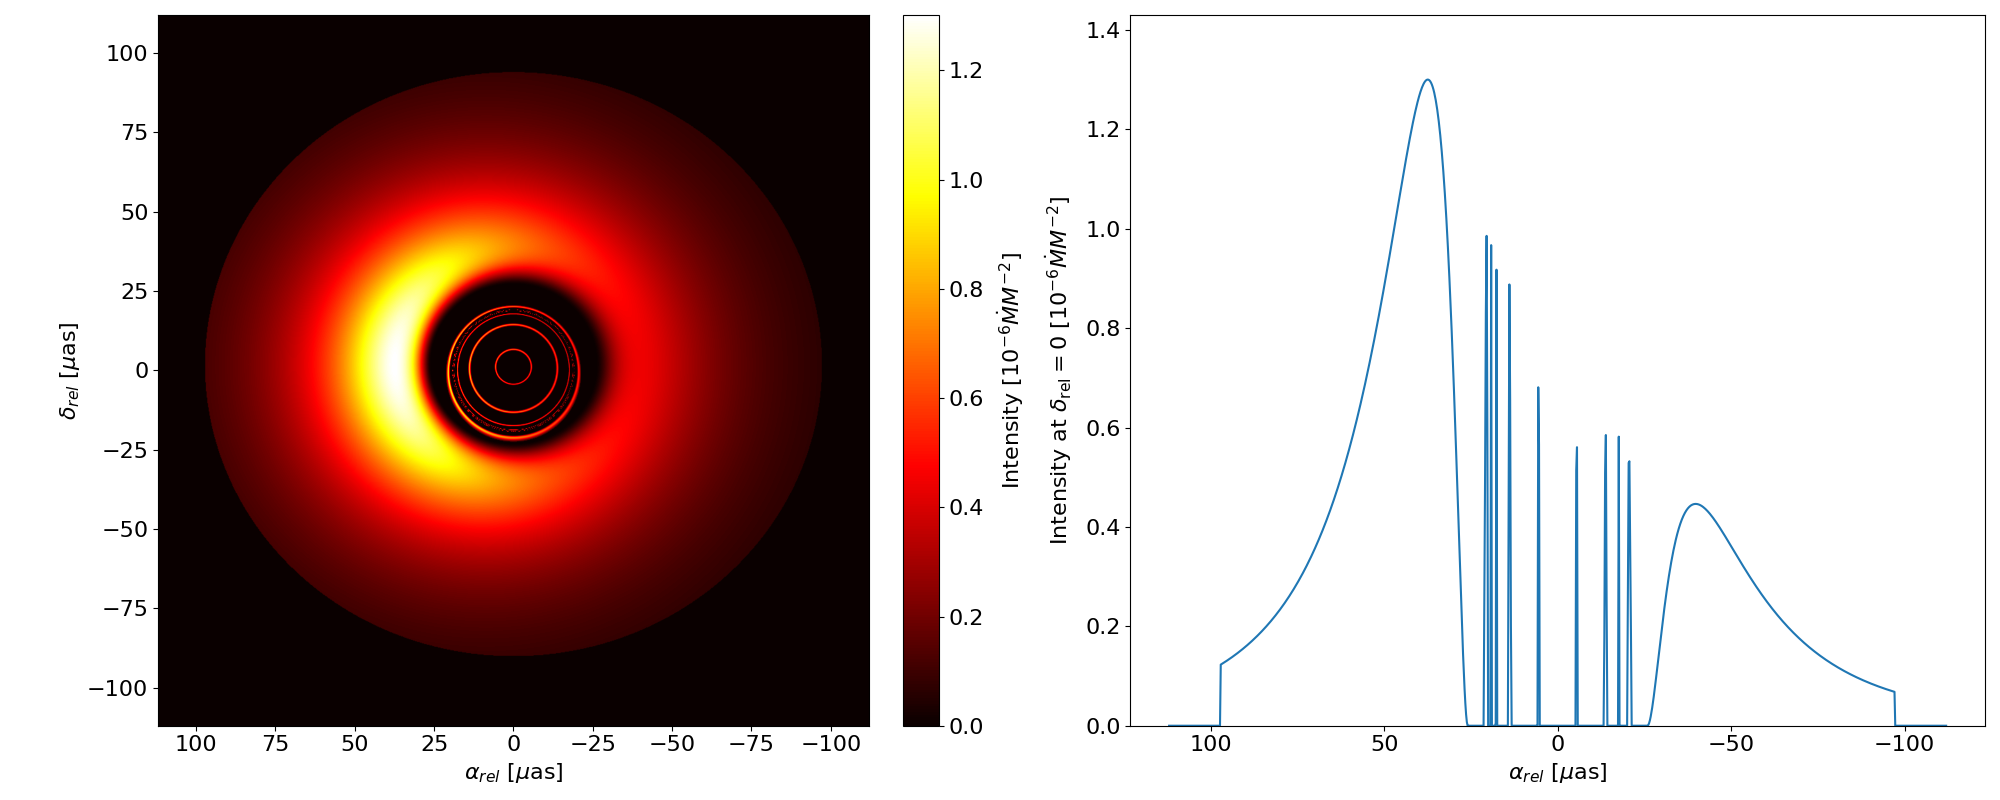
\includegraphics[scale = 0.26]{WH_NT_Gamma2_20_deg.png}
		\caption{$i = 20^\circ$} 
	\end{subfigure}
	\begin{subfigure}{12cm}
		\hspace{-0.6cm}
		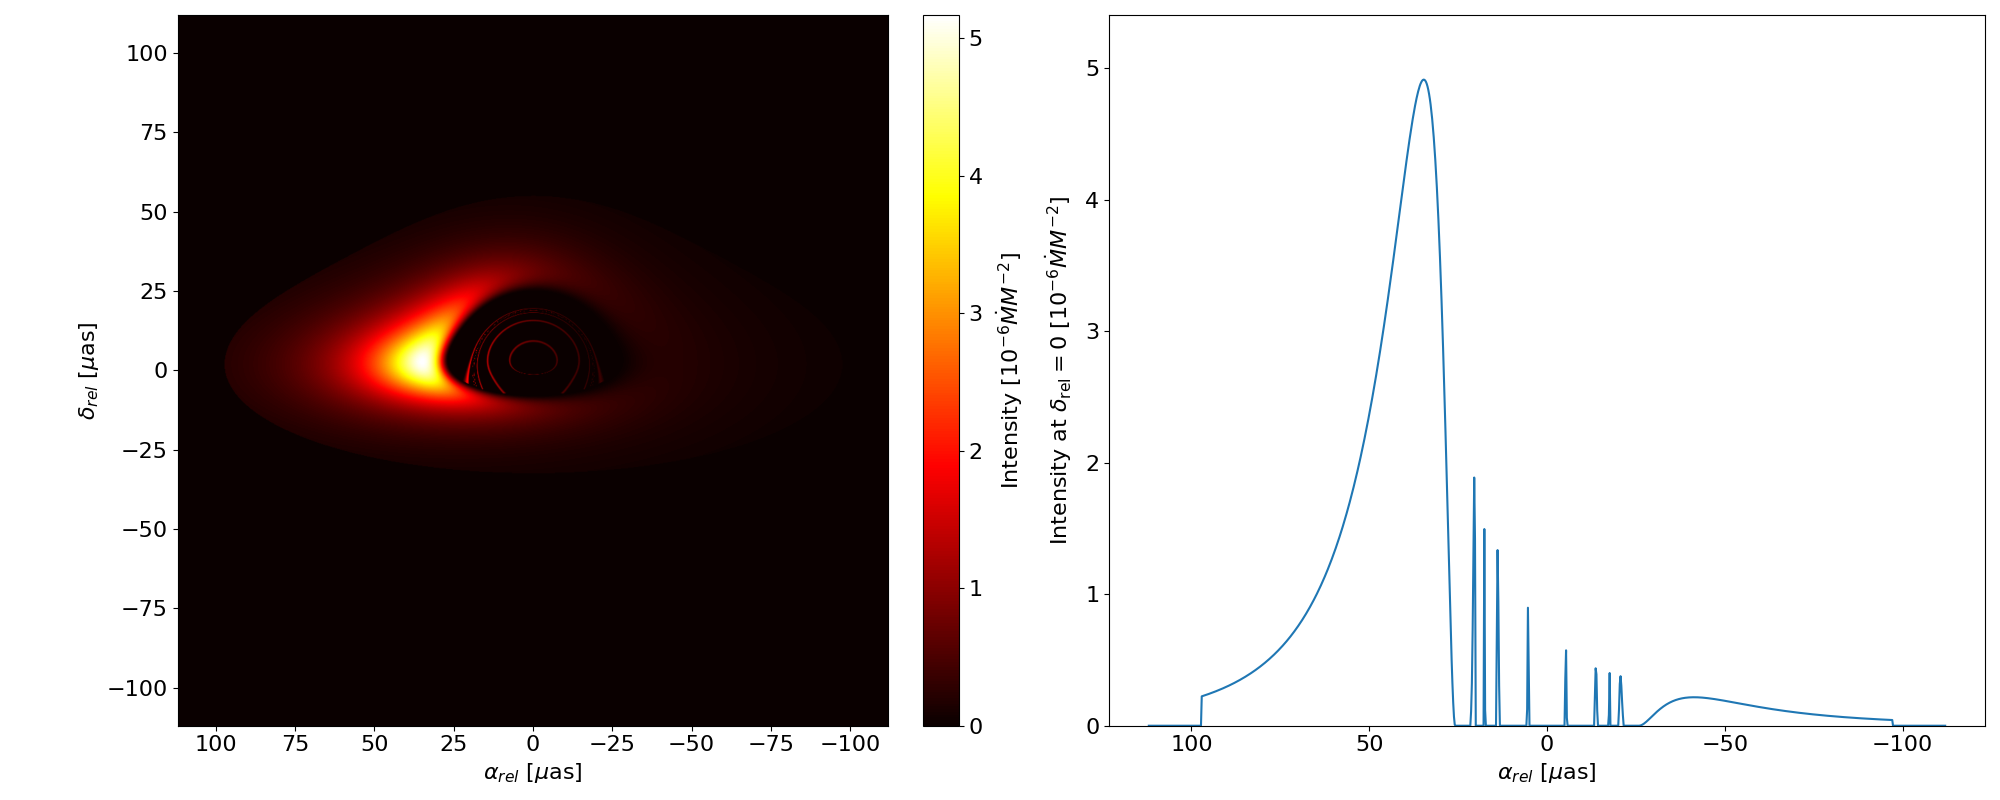
\includegraphics[scale = 0.26]{WH_NT_Gamma2_70_deg.png}
		\caption{$i = 70^\circ$} 
	\end{subfigure}
	\caption[Диск на Новиков-Торн около пространствено-времеви тунел при различни инклинации.]{\small Диск на Новиков-Торн около пространствено-времеви тунел с $\gamma = 2$ при различни инклинации. Параметрите на диска са $r_\text{in} = r_\text{ISCO}$ и $r_\text{out} = 25M$.} 
	\label{WH_NT}
\end{figure}


Виждаме, че при ниски инклинации, централните екзотични образи имат съразмерим интензитет с максимума на целия образ. Докато при високи инклинации, силното доплерово синьо отместване на частта от диска която се движи към наблюдателя доминира, и централните образи са подтиснати с приблизително порядък. Извода, който можем да заключим е, че:\\

\emph{За ниски инклинации, екзотичните образи от пространствено-времеви тунели са \textbf{силно} релевантни за наблюденията, докато при високи, засичането им би било сравнително по-трудно, но не и нереалистично.} \\

Аналогична картинка можем да видим за силни голи сингулярности на Джанис-Нюман-Уиникър, показано на фигура \ref{JNW_NT}, както и за слаби голи сингулярности на Гаус-Боне, показано на фигура \ref{GB_NT}.

\begin{figure}[!htb]
	\centering
	\begin{subfigure}{12cm}
		\hspace{-0.6cm}
		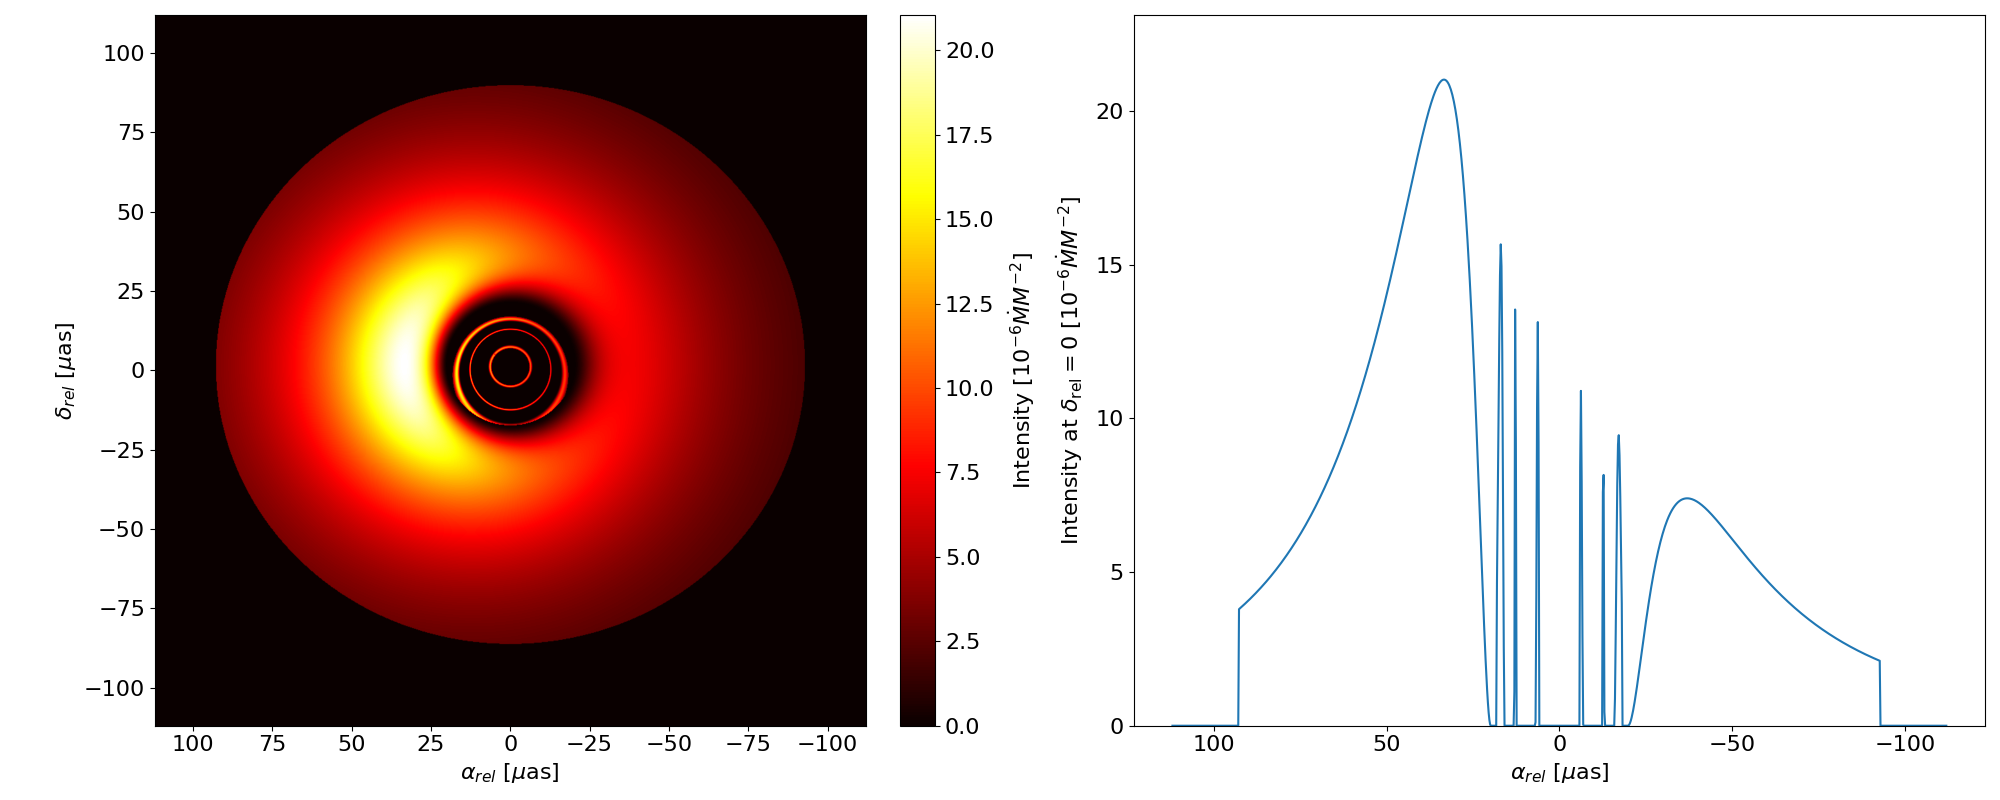
\includegraphics[scale = 0.26]{JNW_NT_Gamma0.48_20_deg.png}
		\caption{$i = 20^\circ$} 
	\end{subfigure}\\
	\begin{subfigure}{12cm}
		\hspace{-0.6cm}
		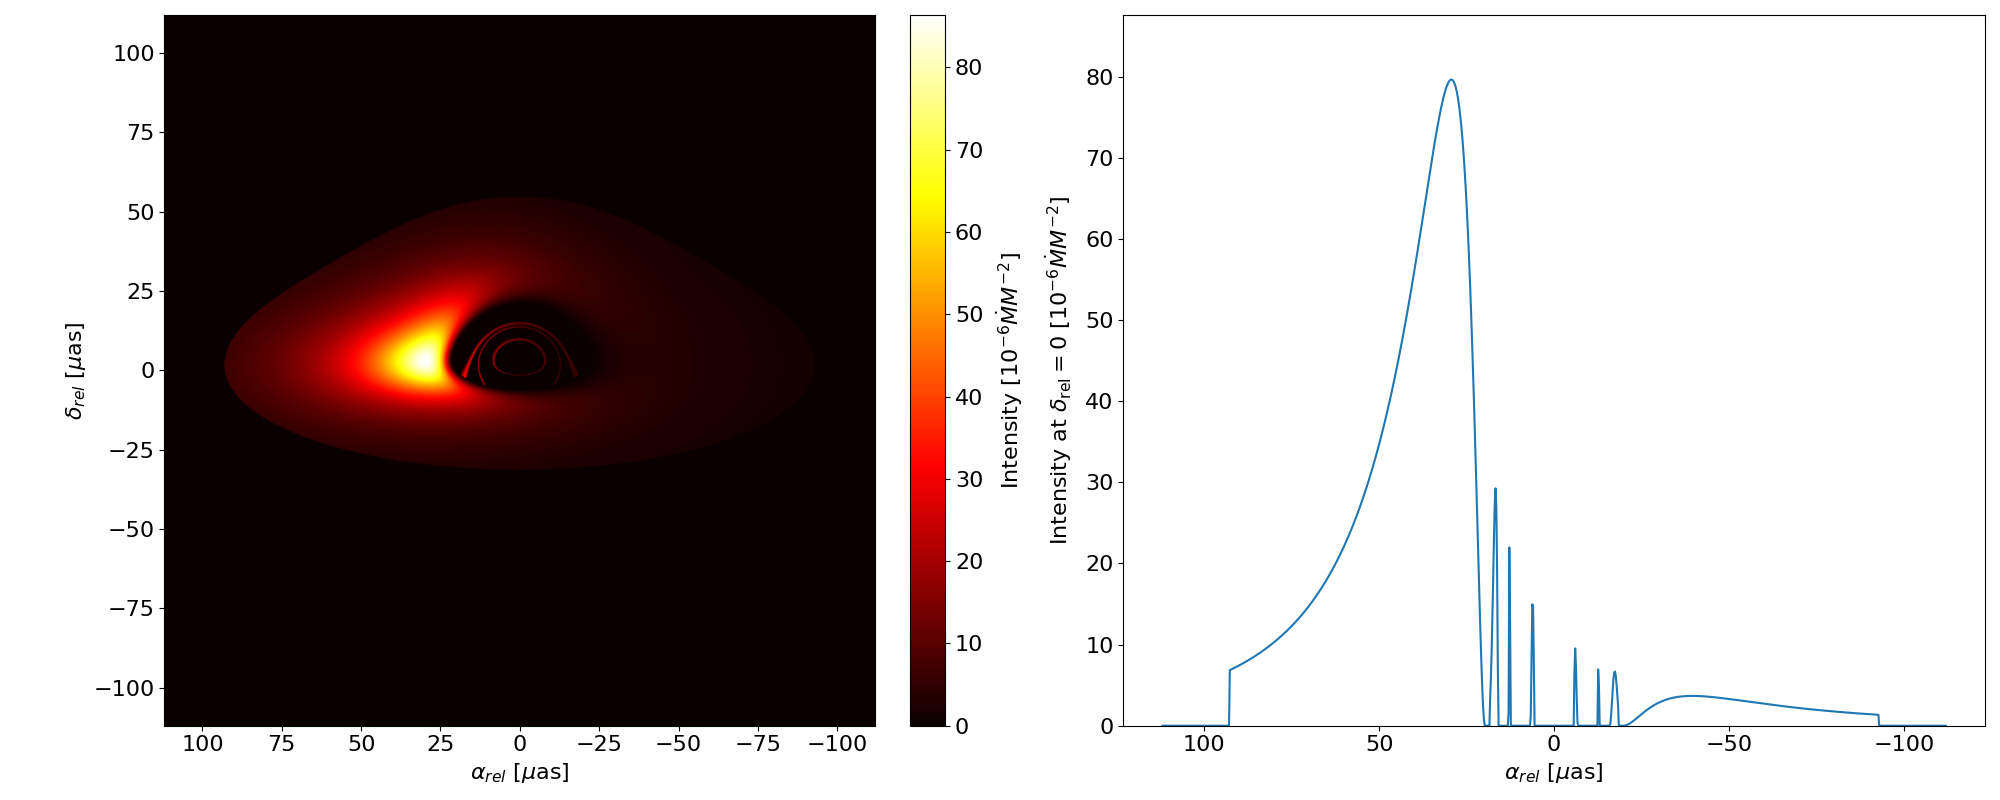
\includegraphics[scale = 0.26]{JNW_NT_Gamma0.48_70_deg.png}
		\caption{$i = 70^\circ$} 
	\end{subfigure}
	\caption[Диск на Новиков-Торн около силни голи сингулярности на Джанис-Нюман-Уиникър при различни инклинации.]{\small Диск на Новиков-Торн около силни голи сингулярности на Джанис-Нюман-Уиникър за $\gamma = 0.48$ при различни инклинации. Параметрите на диска са $r_\text{in} = r_\text{+}$ и $r_\text{out} = 25M$.} 
	\label{JNW_NT}
\end{figure}

Потокът на техните екзотични образи също следва тази зависимост. Тогава на база на тези 3 характерни примера можем да заключим следното:\\

\emph{Морфологичните отклонения (спрямо черни дупки на Кер) на релативистките образи на излъчващата среда около екзотични компактни обекти трябва, в общия случай, да се третират като \textbf{силно} релевантни от наблюдателна гледна точка.}\\
\begin{figure}[!htb]
	\centering
	\begin{subfigure}{12cm}
		\hspace{-0.6cm}
		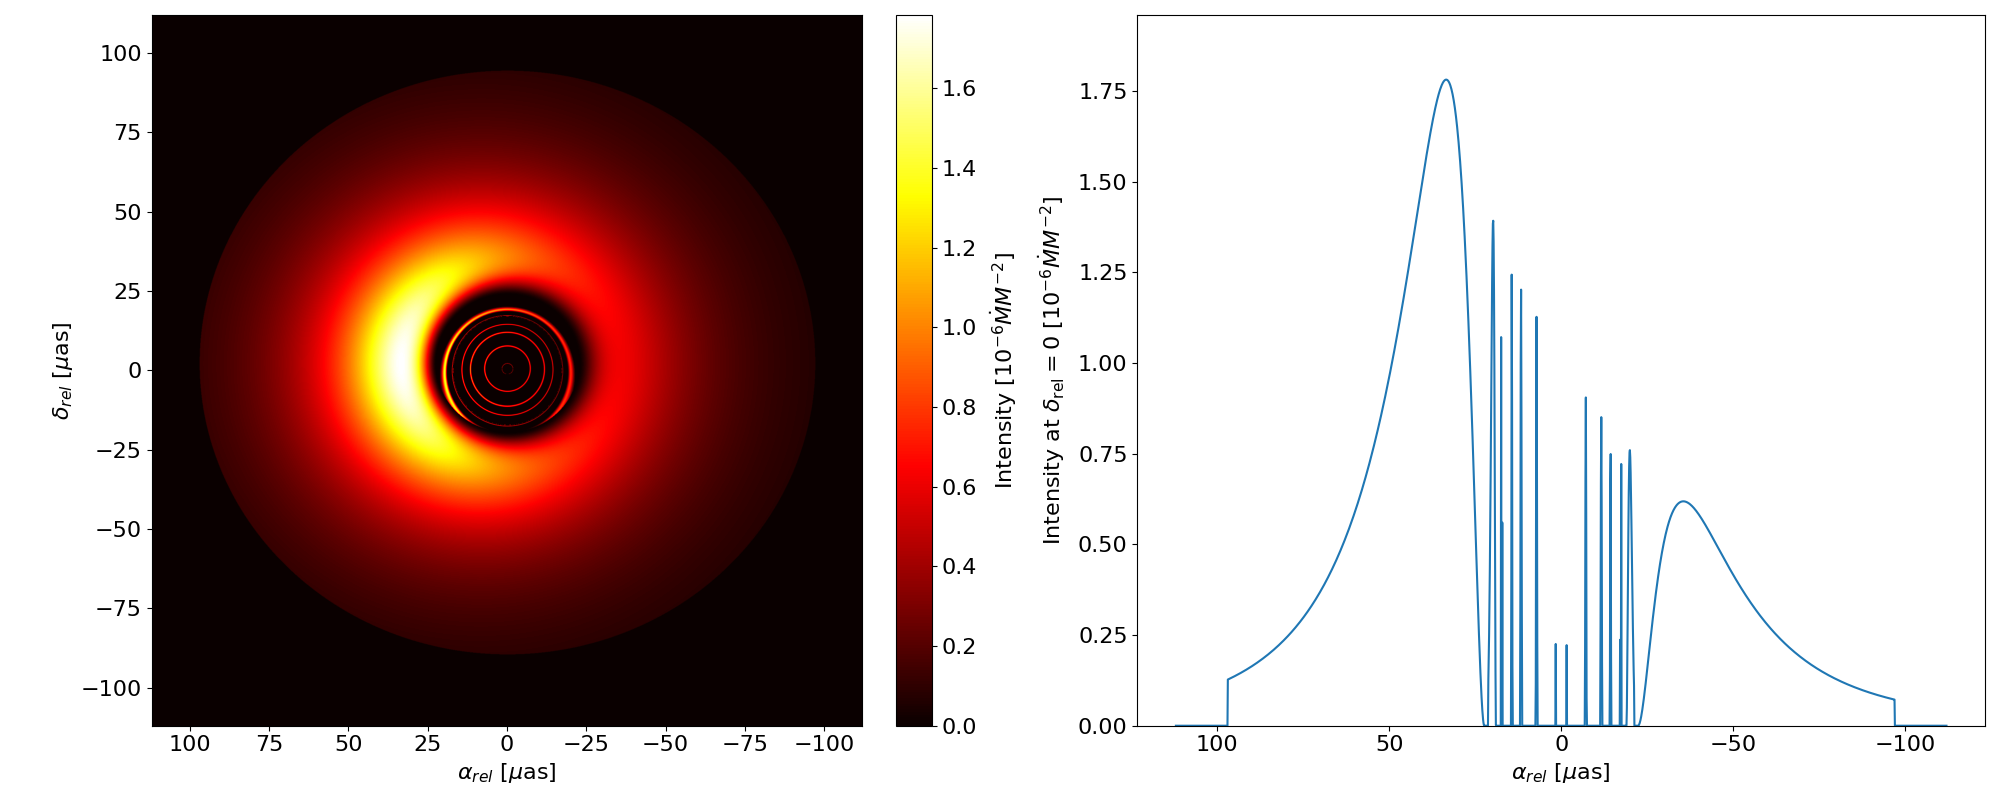
\includegraphics[scale = 0.26]{GB_NT_Gamma1.15_20_deg.png}
		\caption{$i = 20^\circ$} 
	\end{subfigure}\\
	\begin{subfigure}{12cm}
		\hspace{-0.6cm}
		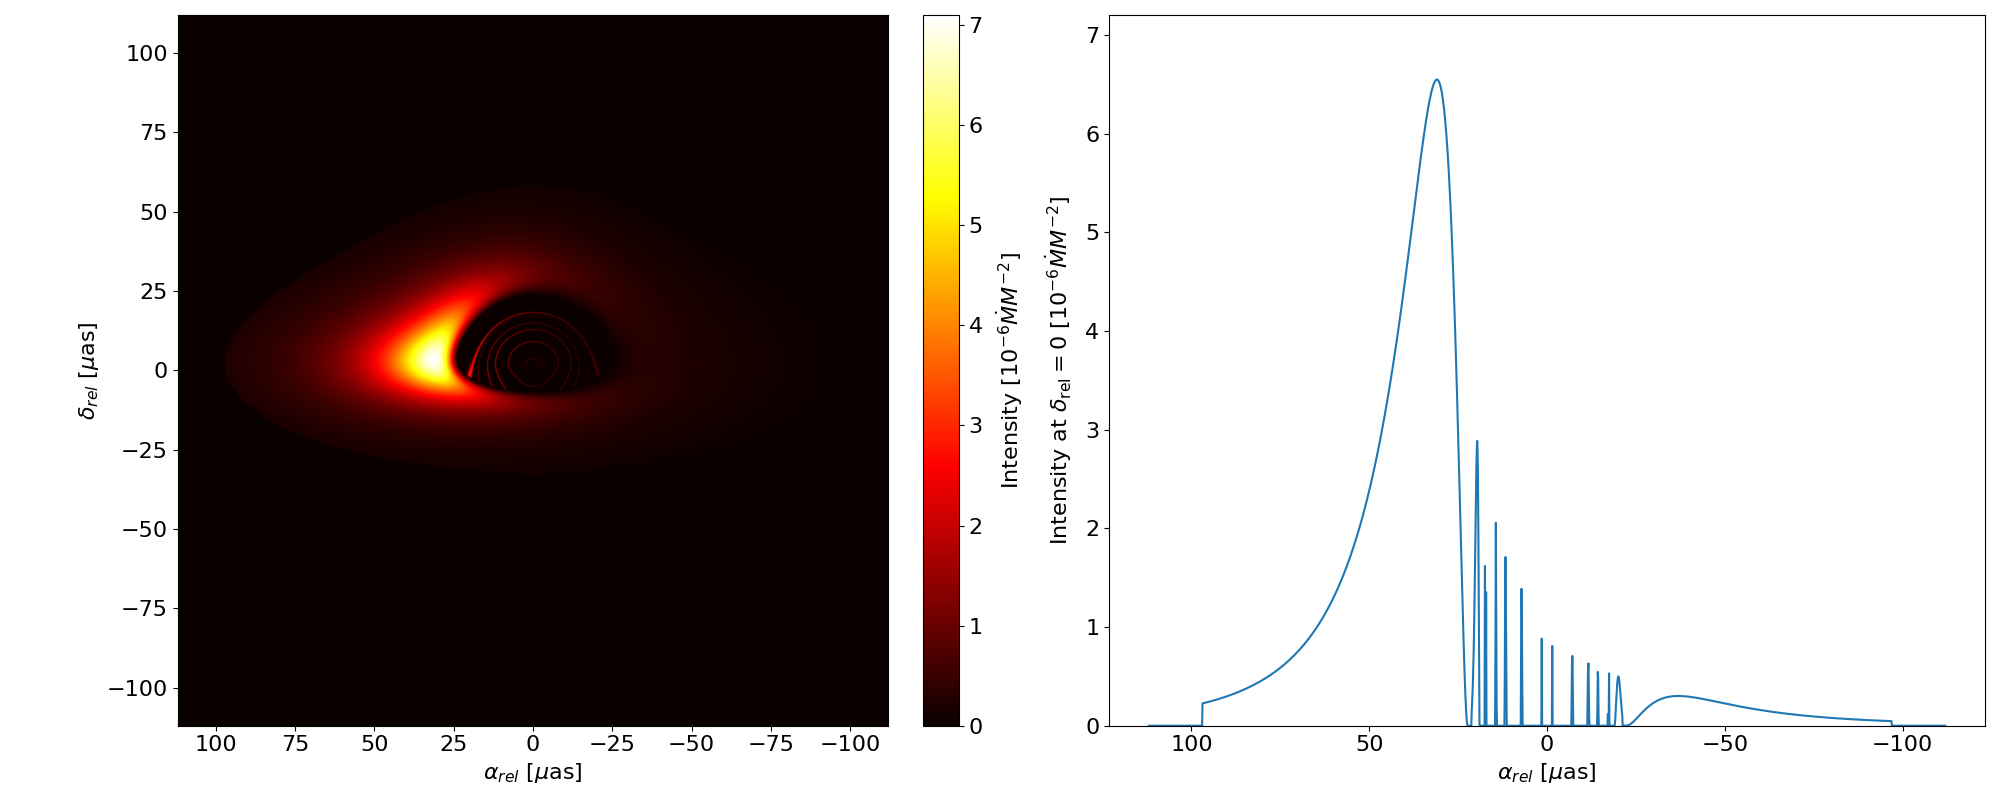
\includegraphics[scale = 0.26]{GB_NT_Gamma1.15_70_deg.png}
		\caption{$i = 70^\circ$} 
	\end{subfigure}
	\caption[Диск на Новиков-Торн около силни голи сингулярности на Гаус Боне при различни инклинации.]{\small Диск на Новиков-Торн около силни голи сингулярности на Гаус-Боне за $\gamma = 1.15$ при различни инклинации. Параметрите на диска са $r_\text{in} = r_\text{+}$ и $r_\text{out} = 25M$.} 
	\label{GB_NT}
\end{figure}

В глава 3 вече обобщихме най-съвременните (до момента на писане) наблюдения на свръхкомпактни обекти от колаборацията EHT. Подобни на тях изследвания в бъдеще имат потенциала за \emph{директно наблюдателно потвърждение за валидността на гравитационни теории отвъд ОТО}. В глава 8 ще изследваме способността на методиката и апаратурата на колаборацията EHT да засече \emph{еднозначно} наличието на подобни образи. За тази цел ще трябва за въведем цялостен, \emph{реалистичен} (за разлика от използваният тук) модел на излъчващата среда. Основните наблюдателни сведения на базата на които ще фиксираме този модел също обсъдихме в глава 3. Едно от тези сведения обаче, заслужава особено внимание - а именно \emph{поляризацията} на светлината от излъчващата среда. Понеже наблюдаваното излъчване идва от зони, много близки до гравитационният център, поляризацията му има потенциалът да кодира изключително богата информация за природата на пространство-времето. Нека преди да се фокусираме върху бъдещите ни наблюдателни способности (глава 8), да разгледаме "отпечатъкът"$\,$ на пространство-времето обект върху поляризацията на лъчението. 




\newpage